\chapter{Implementation}
\label{chap:num_5}

The following chapter is going to cover the implementation of \lpas{} package, the frontend components as well as the ontology. The first part of the chapter dedicated to the implementation of the package will provide a detailed overview of the decisions made on the development stack, the main challenges invoked in refactoring the original \lpa{} codebase, and making the \solid{} related functionality more generic. The frontend components section will dive deeper into the implementation of the mocks provided in \autoref{chap:num_4}, main decisions, and challenges while developing under React. The ontology \autoref{ssec:storage_ontology_implementation} will describe how the designed \lpas{} vocabulary was converted into a OWL file, converted into JSON-LD Schema and later integrated into the \lpa{} frontend. Lastly, an overview of the implementation results will be presented by reiterating over the defined \lpa{} requirements and how they were satisfied by the implementation.
 
\section{Storage Package}
\label{ssec_storage_package_implementation}

The initial implementation of \lpa{} frontend was written in \texttt{JavaScript ES6} \footnote{\url{http://es6-features.org}} and \texttt{React} framework. The development stack also included tools such as \texttt{Babel} \footnote{\url{https://babeljs.io}} compiler and \texttt{Webpack} \footnote{\url{https://webpack.js.org}} package bundler. 

\begin{figure}[h]
\centering
\fcolorbox{black}{white}{
\includegraphics[width=0.4\linewidth]{lpas_package_logo.png}}
\caption{Official \lpas{} package logo designed by author.}
\label{fig:lpas_package_logo}
\end{figure}

As the amount of features and functionality to cover was increasing, the decision was made to separate the \solid{} storage related functionality into a separate npm package and call it \lpas{} package. This section will provide an overview of preliminaries chosen for the implementation of \lpas{} package as well as the specifics of implementations of each abstraction defined in \autoref{ssec:storage}. 

\subsection{Preliminaries}

As briefly mentioned earlier, there are several main libraries used inside the \lpas{} package:

\begin{itemize}
    \item \texttt{rdflib} is a low-level RDF library, that mainly provides the functionality to Read and Write RDF in many popular formats, a querying store and an ability to use SPARQL queries.
    \item \texttt{solid-auth-client}, a browser library that implements \solid{} specifications for providing authentication. This is the main library used to enable the authentication into \lpa{} platform.
\end{itemize}

Due to the complexity of the usage of the stated libraries, specifically \texttt{rdflib}, having an environment and a language that provides a fully-featured object-oriented programming and static type-checking would directly affect the code maintainability and usage. Hence, the codebase of \lpas{} was implemented using \texttt{TypeScript} \footnote{\url{https://www.typescriptlang.org}}. TypeScript is a strict syntactical superset of JavaScript that provides optional static typing and better object-oriented programming capabilities. When referred to files containing TypeScript code, the consecutive sections and chapters will refer to as \textit{TS} files.

\begin{figure}[h]
\centering
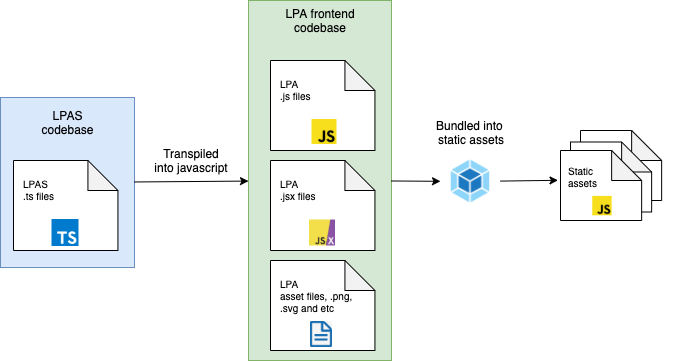
\includegraphics[width=12cm]{lpas_implementation_transpilation_diagram.png}
\caption{A diagram demonstrating the process of transpilation of \lpas{} package and bundling \lpa{} frontend with Webpack}
\label{fig:lpas_implementation_transpilation_diagram}
\end{figure}

As demonstrated on \autoref{fig:lpas_implementation_transpilation_diagram}, integrating the package into the \lpa{} codebase was done using the TypeScript compiler that allows transpilation into ES6 compatible JavaScript syntax. The package, as well as the rest of the \lpa{} codebase,  is later bundled into a set of static assets using Weback. The assets mainly consist of a set of media files such as PNG and SVG files and a large JS file that contains the whole \lpa{} frontend. One of a few disadvantages with that approach is that the initial loading of the frontend might take a few seconds to load in the browser. Afterward, the interaction with the platform is seamless and does not involve any additional loading.

\subsubsection{Project structure}

The structure of the \lpas{} package is simple and straightforward and can be demonstrated as follows:

\begin{listing}[H]    
\begin{minted}[breaklines,frame=single,framerule=1pt,bgcolor=LightGray]{text}
- build       # Transpiled JavaScript code    
- markdown    # Markdown assets
- src         # Root project folder
  - lib       # Main library codebase
    - common  # Utilities and helper functions
       - ...     # TypeScript tests and core abstractions
  - types     # Custom user-defined type definitions
- docs        # Static html with library documentation
_ ...         # Readme and various configuration files
\end{minted}
\caption{\lpas{} package folder structure description.} 
\label{lst:lpas_folder_structure}
\end{listing}

The proceeding sections will describe the individual abstractions mentioned in \autoref{ssec:storage}.

\subsection{Authentication Manager}
\label{sssec:authentication_manager_implementation}

This section will continue the architectural description of the Authentication manager described in \autoref{sssec:authentication_manager}, describe the implementation, and provide examples of how the abstraction is used inside \lpa{}.

The \textit{AuthenticationManager} is a Singleton class, instantiated only once and utilized both in the package itself as well as being invoked from \lpa{} frontend codebase. The reason for the class being implemented as a singleton is due to the fact that it wraps the functionality of \texttt{solid-auth-client} library, and it provides a singleton instance as well. Aside from providing the WebID authentication,  \texttt{solid-auth-client} implements a WebID OIDC specific \textit{fetch} functionality. The \textit{FETCH API} is originally a JavaScript API that provides an ability to send asynchronous HTTP calls. The implementation in \texttt{solid-auth-client}, is based on \texttt{isomorpic-fetch}, which is a third party framework that implements the \textit{Fetch API} both for browsers and Node.js. Hence, the abstraction is used for:
\begin{itemize}
    \item Authentication, and ability to track the user session with callbacks. 
    \item Sending HTTP calls to \solid{} server.
\end{itemize}


\begin{figure}[h]
\centering
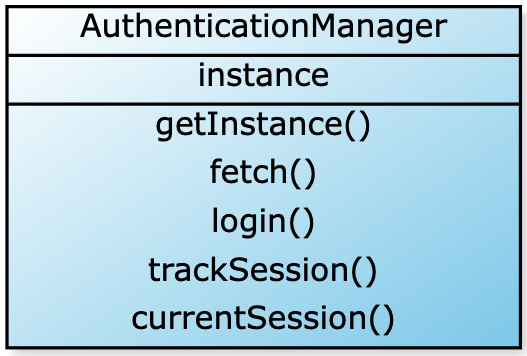
\includegraphics[width=6cm]{lpas_authentication_class.png}
\caption{A class diagram generated directly from a TypeScript file, demonstrating an implemented \textit{AuthenticationManager} abstraction}
\label{fig:lpas_authentication_class}
\end{figure}


In other words, once the client is logged in the \solid{} app, consecutive interactions are performed via \textit{fetch} function that is conveniently wrapped in the \textit{AuthenticationManager} abstraction.

As demonstrated on \autoref{fig:lpas_authentication_class}, the class consist of a set of public methods described as follows:
\begin{itemize}
    \item \textit{getInstance()}, this public method returns a singleton instance to an AuthenticationManager.
    \item \textit{fetch()}, a wrapper redirecting the call to \texttt{solid-auth-client} fetch method.
    \item \textit{login()}, a wrapper redirecting the call to \texttt{solid-auth-client} login method.
    \item \textit{trackSession()}, a method with asynchronous callback notifying the listener when a logout or login operation is performed.
    \item \textit{currentSession()}, a method returning the instance of a \texttt{solid-auth-client} Session object that contains relevant information about the authenticated user and his WebID. 
\end{itemize}

Referring back to \autoref{fig:lps_authentication_sequence_diagram}, there are several places in \lpa{} codebase where the \textit{AuthenticationManager} is invoked directly. The implementation of React components will be covered in the proceeding section, but the invocation of the abstraction itself can be described as follows:
\begin{itemize}
    \item \textit{Component layouts} are special high-level react containers that wrap every other container inside \lpa{} frontend. They are differentiated by \textit{public} and \textit{private}. The \textit{private} components reactively monitor the authenticated session of a user and redirect them back to the authentication screen whenever the value of the session becomes \texttt{undefined}. It is important to note that the session object from \textit{AuthenticationManger} is duplicated in \lpa{} frontend as a Redux state. Therefore, any changes in the original session object are reflected on that state and triggers re-rendering of layout components. 
    \item \textit{Authentication component functions}, are the functions being invoked when user attempts to perform the authentication. In other words, this is the input that triggers the flow demonstrated earlier on \autoref{fig:lps_authentication_sequence_diagram}.
    \item \textit{The App router}, the main class in \lpa{} that serves as an entry point and utilizing the \texttt{react-router} \footnote{\url{https://www.npmjs.com/package/react-router}} package, contains a function that invokes the \textit{trackSession()} method in \textit{AuthenticationManager}. This directly links to the session object and updates the changes from original session to internal Redux state.
\end{itemize}

The usage of both \textit{currentSession()} and \textit{login()} methods from \textit{AuthenticationManager} can be observed below:

\begin{listing}[H]    
\begin{minted}[breaklines,frame=single,framerule=1pt,bgcolor=LightGray]{javascript}
login = async (idp, callbackUri) => {
    const session = await AuthenticationManager.currentSession();
    if (!session)
      await AuthenticationManager.login(idp, {
        storage: localStorage
      });
    else {
      Log.info(`Logged in as ${session.webId}`);
      return session;
    }
};
\end{minted}
\caption{An implementation of \textit{login()} wrapper.} 
\label{lst:lpas_login_wrapper}
\end{listing}

To sum up, the \textit{AuthenticationManager} is a simple and straightforward singleton abstraction that wraps the \texttt{solid-auth-client} library and only necessary functions from the wrapped library to be used inside \lpas{} package. The examples of invocation from within the \lpas{} package are limited to directly calling the \textit{fetch()} method whenever a HTTP request is assembled and needs to be executed, more details on that will be described in a section dedicated to \textit{FileManager} abstraction.  

\subsection{File Manager}
\label{sssec:file_manager_implementation}

In this subsection, we will continue on the \textit{FileManager} abstraction described in \autoref{sssec:file_manager}, provide the specifics on implementation as well as a detailed overview of each method inside the abstraction.  

\begin{figure}[h]
\centering
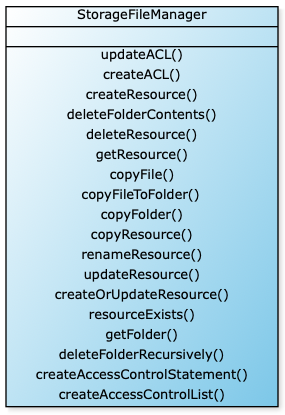
\includegraphics[width=5cm]{lpas_implementation_file_manager_diagram.png}
\caption{A class diagram generated directly from a TypeScript file, demonstrating an implemented \textit{FileManager} abstraction}
\label{fig:lpas_filemanager_implementation_class}
\end{figure}

Similar to the \textit{AuthenticationManager}, the \textit{FileManager} abstraction is implemented as a TypeScript class providing a set of public static methods. It is responsible for all core \textit{CRUD} operations with \solid{} resources. It is important to note that all HTTP requests to \solid{} server are made using the \textit{fetch()} method invoked via \textit{AuthenticationManager}. In other words \textit{FileManager} relies on \textit{AuthenticationManager} when performing HTTP requests. To follow up a class representation on \autoref{fig:lpas_filemanager_implementation_class}, the methods can be described as follows:
\begin{itemize}
    \item \textit{createResource()}, a function is responsible for creating new \solid{} resources. 
    \item \textit{deleteFolderContents()}, a function is mainly used for cleaning up the content of a particular folder. It iterates the contents and recursively deletes underlying folders and files.
    \item \textit{deleteResource()}, a function responsible for deleting individual resources from a \solid{} POD. Following the sequence flow presented on \autoref{fig:lps_rename_resource}, depending on the type of the resource it will either remove it directly or attempt to clean it recursively if the resource is an \textit{LDP-BC}.
    \item \textit{getResource()}, a basic function executing a GET call to obtain a resource content from a \solid{} server.
    \item \textit{copyFile()}, a basic function performing a copy operation on an \textit{LDPR}.
    \item \textit{copyResource()}, a generic method performing a copy operation on a resource. Depending on the type of the resource it either invokes the \textit{copyFile()} directly or, if resource is an \textit{LDP-BC}, it performs a recursive copying.
    \item \textit{renameResource()}, a method responsible for changing the title of the resource inside the \solid{} POD. In that case it simply means changing the absolute path to resource, where the name is the last element in the path. This function is described in detail on \autoref{ssssec:renaming_resources}. The operation involves invocation of several simpler methods from the \textit{FileManager} abstraction.
    \item \textit{updateResource()}, a generic function executing an HTTP PUT request for a particular resource.
    \item \textit{createOrUpdateResource()}, a method used in cases when a resource needs to be updated even if a different resource exists under that path. If a nothing exists under supplied path, resource will be created, if an object exists under particular path then it will be removed first.
    \item \textit{resourceExists()}, a method that executes the HTTP GET call to check if anything exits under specified path. The response is a simple boolean value.
    \item \textit{getFolder()}, a method that parses the contents of a particular folder and returns it as an array of underlying files and folders wrapped into a simple configuration abstraction. This is mainly used a part of any recursive operations involving folders.
    \item \textit{deleteFolderRecursively()}, a method used to execute recursive deletion of a particular folder. This is demonstrated in detail on \autoref{fig:lps_delete_resource} under a conditional block that is executed when resource is a folder.  
    \item \textit{createAccessControlStatement()}, \textit{createAccessControlList}, \textit{updateACL()}, \newline{} \textit{createACL()}, following methods can be found described in \autoref{sssec:access_control_manager_implementation}, as they relate to interacting with ACL resources.
\end{itemize}

It is important to note that the class is not a singleton in contrast with \textit{AuthenticationManager}. This is because all classes are exposed as public and static. The design makes the abstraction generic for many use cases within and outside the bounds of requirements of \lpa{}.

The \solid{} resource within the \lpas{} package is represented by \textit{ResourceConfiguration} abstraction that is a basic required input for most of the operations in \textit{FileManager} that involve execution of HTTP requests. The proceeding \autoref{ssssec:lpas_resource_config_implementation} will provide more details on implementation of this class and the relation to \textit{FileManager}.
 
\subsubsection{Resource Configuration}
\label{ssssec:lpas_resource_config_implementation}

One of the challenges when \lpa{} frontend initially contained the code for \solid{} interaction inside was the lack of any abstraction representing a particular \solid{} resource. There were several refactoring attempts to add basic ES6 classes, but maintaining the codebase was not trivial at all. Therefore, after introducing the \lpas{} package, the implementation of abstractions to represent the \solid{} resources was one of the first challenges. The \autoref{fig:lpas_resource_config_implementation} consist of two main entities:
\begin{enumerate}
    \item \textit{ResourceConfig}, a main class representing \textit{ResourceConfiguration} abstraction. 
    \item \textit{SolidResource}, an interface required for each object representing the \solid{} resource to be conforming to. 
\end{enumerate}

\begin{listing}[H]    
\begin{minted}[breaklines,frame=single,framerule=1pt,bgcolor=LightGray]{javascript}
enum SolidResourceType {
  Folder = '<http://www.w3.org/ns/ldp#BasicContainer>; rel="type"',
  File = '<http://www.w3.org/ns/ldp#Resource>; rel="type"'
}
\end{minted}
\caption{Definition of \textit{SolidResourceType} enumerator.} 
\label{lst:lpas_resource_type_enum}
\end{listing}

The \textit{SolidResource} interface consist of the following:
\begin{itemize}
    \item \textit{type}, an enumerator property represented on \autoref{lst:lpas_resource_type_enum}. Type is either a \textit{Folder} or a \textit{File}.
    \item \textit{path}, a \texttt{string} property representing a full absolute path excluding the filename itself. The reason why filename is excluded is to simplify the interactions within \textit{FileManager} class and provide more flexibility when operating with resources.
    \item \textit{title}, a \texttt{string} property representing the tile of the resource. The extension of the resource is not included.
    \item \textit{contentType}, an optional \texttt{string} property representing the content type header to be passed when constructing and HTTP request to  manipulate this resource. If value is not provided, a TTL extension is used by default.
    \item \textit{body}, an optional \texttt{string} property holding a content of the resource. The property is marked optional because there are cases when an empty folder resource need to be created, from an \lpa{} developer point, he does not need to provide any content to create an empty folder resource.
    \item \textit{isPublic}, an optional \textit{boolean} indicating whether the file is controlled only by the creator, owner or can have public read access. This is closely related to \textit{AccessControlManager} abstraction described in \autoref{sssec:access_control_manager_arch}. The proceeding section will describe the implementation of that abstraction in detail.  
\end{itemize}

The fact that \textit{SolidResource} is represented as the interface allows the objects conforming to eat to be constructed effortlessly and straightforwardly, similar to simply creating a \texttt{dictionary} object. The \textit{ResourceConfig}, on the other hand, wraps the object by providing additional information and functionality on top of the original resource object. The \textit{ResourceConfig} class consist of the following:
\begin{itemize}
    \item \textit{webID}, is a \texttt{string} property. The value should be assigned to the creator or owner of the resource. Within \lpa{} frontend, this value is usually holding the \textit{WebID} of the authenticated platform user.  
    \item \textit{resource}, is an \texttt{object} property conforming to \textit{SolidResource} interface. 
    \item \textit{fullPath}, a method returning a concatenated \texttt{string}, representing an absolute path to a resource.
    \item \textit{fullPathWithAppendix()}, a method returning a concatenated \texttt{string}, representing an absolute path to a resource with a \texttt{'/'} symbol. This is required in cases when an operation needs to be performed on a resource a developer wants to be sure that the absolute path will be constructed correctly for the underlying type. The \textit{folder} resource requires the symbol to be appended when dealing with the construction of ACL files. This will be described in more detail in the proceeding section dedicated to \textit{AccessControlManager} abstraction.
\end{itemize}

\begin{figure}[h]
\centering
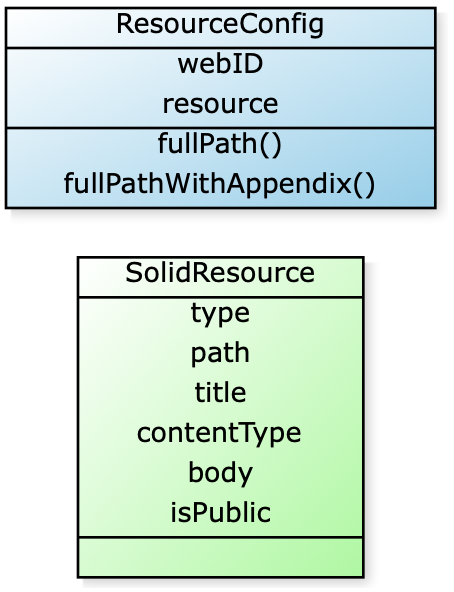
\includegraphics[width=5cm]{lpas_resource_config_implementation.png}
\caption{A class diagram generated directly from a TypeScript file, demonstrating implemented \textit{ResourceConfig} class and \textit{SolidResource} interface}
\label{fig:lpas_resource_config_implementation}
\end{figure}


The \textit{FileManager} class is extensively used throughout the whole \lpa{} frontend codebase. The examples below demonstrated various examples of invocations of the \textit{FileManager} abstraction from within the \lpa{} frontend codebase. It is important to note that the provided examples are generic enough to be applied to the development of any \solid{} application supporting the current iteration of \texttt{node-solid-server}.

\subsubsection{An example on creating a resource}

The example below demonstrated a simple use case on how \lpas{} package can be used to create a \solid{} resource using the \textit{FileManager} abstraction. 

\begin{listing}[H]    
\begin{minted}[breaklines,frame=single,framerule=1pt,bgcolor=LightGray]{javascript}
const folderConfig: ResourceConfig = new ResourceConfig(
        {
          path: rootResourceConfig.fullPath(),
          title: 'configurations',
          type: SolidResourceType.Folder
        },
        webId
      );
      
const response = await StorageFileManager.createResource(folderConfig)
\end{minted}
\caption{An example usage of \textit{FileManager} abstraction to create a folder in \solid{} pod.} 
\label{lst:resource_generation_example}
\end{listing}

In this particular case, a folder resource \textit{ResourceConfig} class instance is being created named \textit{configurationsFolderConfig}. Afterwards it is being passed to a public static \textit{createResource()} method that creates the resource as described on \autoref{fig:lpas_create_resource}. This concludes the description of the implementation of \textit{FileManager} abstraction. The proceeding section is dedicated to an \textit{AccessControlManager} abstraction, following up the first introduction in the \autoref{sssec:access_control_manager_arch}.


\subsection{Access Control Manager}
\label{sssec:access_control_manager_implementation}

This subsection provides details on implementation of the \textit{AccessControlManager} abstraction from \autoref{sssec:access_control_manager_arch} section. Despite being called a separate abstraction, it is in fact implemented as a set of additional public static methods inside the \textit{FileManager} abstraction as seen on \autoref{fig:lpas_filemanager_implementation_class} diagram. Essentially every ACL resource is yet another resource represented as \textit{LDPR} in \solid{}. However the functional implication of those resource are more specific and require extra information and functionality to operate with them. That is why it is separated conceptually as a different abstraction but is implemented inside the same class called \textit{FileManager}. 

Referring back to \autoref{fig:lpas_filemanager_implementation_class}, the main methods related to the abstraction are described as follows:
\begin{itemize}
    \item \textit{updateACL()}, a method constructing the array of RDF triples that is later serialized into a TTL and send as a body in HTTP PUT request to \solid{} server, replacing the previous resource under that path.
    \item \textit{createACL()}, a method constructing the array of RDF triples that is later serialized into a TTL and send as a body in HTTP PUT request to \solid{} server.
    \item \textit{createAccessControlStatement()}, a method constructing the array of RDF triples expressing access control for a particular WebID. 
    \item \textit{createAccessControlList()}, a method assembling an array of access control statements for multiple requested WebIDs using \textit{createAccessControlStatement()}, and as result serializes the array of statements into a raw TTL \texttt{string} using \texttt{rdflib}.
\end{itemize}

The functionality implemented by \textit{AccessControlManager} is not conforming to entire Web Access Control specification, since it was not needed and not required to satisfy the \lpa{} requirements. Therefore, methods described earlier such as \textit{updateACL()} and \textit{createACL()} as seen on \autoref{fig:lps_acl_update_flow}, were based on the default ACL files that \texttt{NSS} generates. At the moment of writing this thesis, the default ACL files generated by \texttt{NSS v5.2.0} looks as follows:

\begin{listing}[H]    
\begin{minted}[breaklines,frame=single,framerule=1pt,bgcolor=LightGray]{turtle}
@prefix : <#>.
@prefix n0: <http://xmlns.com/foaf/0.1/>.
@prefix n1: <http://www.w3.org/ns/auth/acl#>.
@prefix test: <./>.
@prefix c: </profile/card#>.
 
:owner
    n1:accessTo test:;
    n1:agent c:me;
    n1:default test:;
    n1:mode n1:Control, n1:Read, n1:Write.
:public
n1:accessTo test:; n1:agentClass n0:Agent; n1:default test:; n1:mode n1:Read.
\end{minted}
\caption{An example ACL resource in TTL describing access control for a folder} 
\label{lst:acl_file_example}
\end{listing}

As seen on \autoref{lst:acl_file_example}, the example describes access control privileges to a folder named \textit{test}. The first semantic triple contains a subject named \texttt{:owner}, and this refers to the WebID of the owner of this \solid{} POD. The predicates of the Owner subject can be described as follows:
\begin{itemize}
    \item \textit{accessTo}, the information resource to which the access is being granted. In this case, we are granting access to a folder named \textit{test}
    \item \textit{agent}, a person or an entity to whom the rights are being given. Since this is an owner of the \solid{} pod, the reference is given to himself.
    \item \textit{default}, this is a special predicate that behaves as follows. If the underlying resources have no ACL files specified they would keep referring to parent resources until it will reach the resource containing the ACL file with \textit{default} predicate. In this case, the statement says that the underlying resources without explicitly set ACL files will have the same access control rights as the \textit{test} folder.
    \item \textit{mode}, a predicate describing the access control modes. In this case, the object is defined as follows: 
        \subitem \textit{Control}, a semantic object describing full read and write access to an ACL of the resource.
        \subitem \textit{Read}, a semantic object, is giving full read access to a resource.
        \subitem \textit{Write}, a semantic object is giving full write access to a resource.
\end{itemize}

On the other hand, the subject named \textit{public} only has an ability to \textit{Read} the folder and its content. The \textit{public} subject is just a generic simplification for cases when there is no need to set specific WebIDs explicitly. However, using ACL easily allow listing particular users as well, giving a lot of flexibility to have a very sophisticated access control privileges setup per any resource in a \solid{} POD. As mentioned earlier, the ability to manipulate access control to any resource and own your data is one of the core benefits proposed by \solid{} project. 

\subsubsection{Access Control Configuration}

Aside from the main \textit{AccessControlManager} abstraction, as demonstrated on \autoref{chap:num_1}, the original \textit{ResourceConfig} class from \textit{FileManager} required to be extended by introducing several subclasses called:
\begin{itemize}
    \item \textit{AccessControlConfig}, a subclass of \textit{ResourceConfig} that adds a property listing available control modes to a resource for specified WebID, and adds methods to construct the proper absolute path to a resource. The only difference between those methods and methods described in \autoref{ssssec:lpas_resource_config_implementation} such as \textit{fullPath()} and \textit{fullPathWithAppending()}, is that the hardcoded keyword ACL for files and hardcoded keyword \texttt{/.acl} for folder are being appended.
    \item \textit{AccessControlStatementConfig}, a subclass of \textit{AccessControlConfig}, contains additional references to \texttt{rdflib} nodes to simplify construction of ACL triples in \textit{AccessControlManager} abstraction.
\end{itemize}

\begin{figure}[h]
\centering
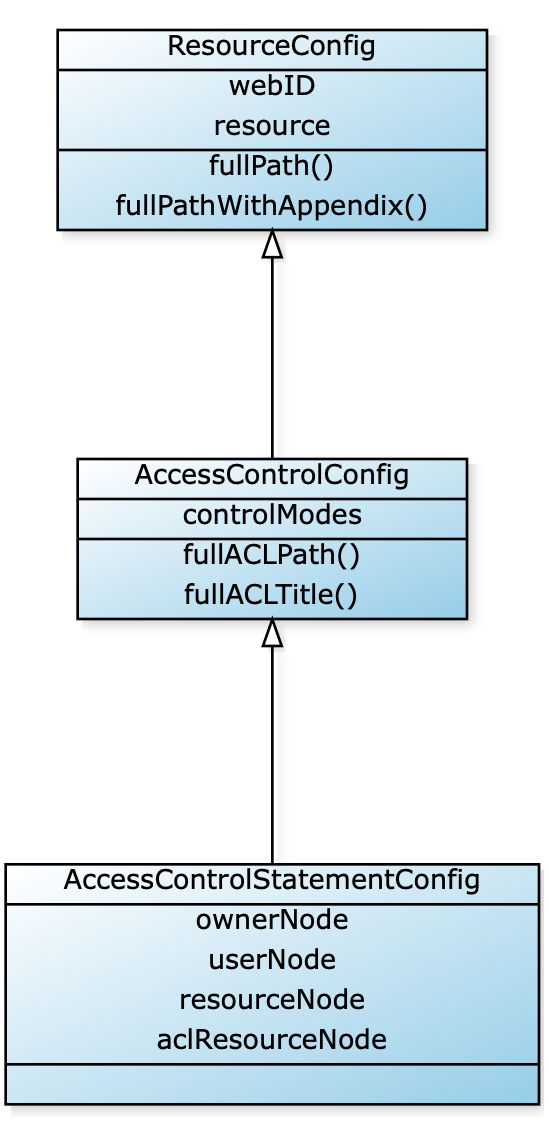
\includegraphics[width=4cm]{lpas_access_control_config_imlementation.png}
\caption{A class diagram generated directly from a TypeScript file, demonstrating implemented \textit{AccessControlConfig} and \textit{AccessControlStatementConfig} extending \textit{ResourceConfig}}
\label{fig:lpas_access_control_config_imlementation}
\end{figure}

\subsubsection{An example on creating an ACL file for a \solid{} resource}

The example below demonstrated a simple use case on how \lpas{} package can be used to create an ACL file for a \solid{} resource using the \textit{FileManager} abstraction. 

\begin{listing}[H]    
\begin{minted}[breaklines,frame=single,framerule=1pt,bgcolor=LightGray]{javascript}
const configurationsAclResourceConfig: AccessControlConfig = new AccessControlConfig(
  {
    ...configurationsFolderConfig.resource,
    isPublic: true
  },
  [AccessControlNamespace.Read, AccessControlNamespace.Write],
  webId
);

const response = await StorageFileManager.updateACL(
  configurationsAclResourceConfig
);
\end{minted}
\caption{An example ES6 code on creating ACL files for \solid{} resource in \lpa{} frontend} 
\label{lst:acl_creation_lpa_example}
\end{listing}

In this case, a folder resource is expressed as a \textit{ResourceConfig} class instance under \textit{configurationsFolderConfig} constant and \textit{configurationsAclResourceConfig} constant is created based on it to express and ACL file. Using the ES6 \texttt{spread} operator we populate the description of the folder resource as follows '\texttt{...configurationsFolderConfig.resource}'. Afterwards, the access control modes are supplied in an array giving the ability to \textit{Read} and \textit{Write} to that resource to anyone by default. In the last step the specify the webId of the owner of the resource and the ACL file to be created and supply the constructed \textit{AccessControlConfig} into \textit{updateACL()} method that is demonstrated in detail on this sequence \autoref{fig:lps_acl_update_flow}.

To sum up, the section provided an overview of three main abstractions inside \lpas{} package. The \textit{AuthenticationManager} used as a main class to deal with WebID based authentications for \lpa{} platform. The \textit{FileManager}, responsible for managing all HTTP requests to manipulate resources in a \solid{} resource. \textit{AccessControlManager} abstraction that significantly simplified the interactions with \solid{} inside \lpa{} frontend significantly and gave an ability to implement more advanced access control related features to configure the published \lpa{} visualizers. This will be demonstrated in detail in \autoref{sssec:lpas_storage_frontend_implementation}. The consequitive section will describe the \lpas{} Ontology originally described in \autoref{fig:lps_acl_update_flow}, its implementation and hosting.

\section{Hosting Storage Ontology}
\label{ssec:storage_ontology_implementation}

This section is going to continue the details on implementation of the \lpas{} ontology, firstly described in \autoref{ssec:lpas_application_ontology_arch}. As mentioned earlier, the intent to design the ontology was to utilize the benefits of \solid{} better and the ways in which every entity is represented as an RDF resource.

\begin{figure}[h]
\centering
\fcolorbox{black}{white}{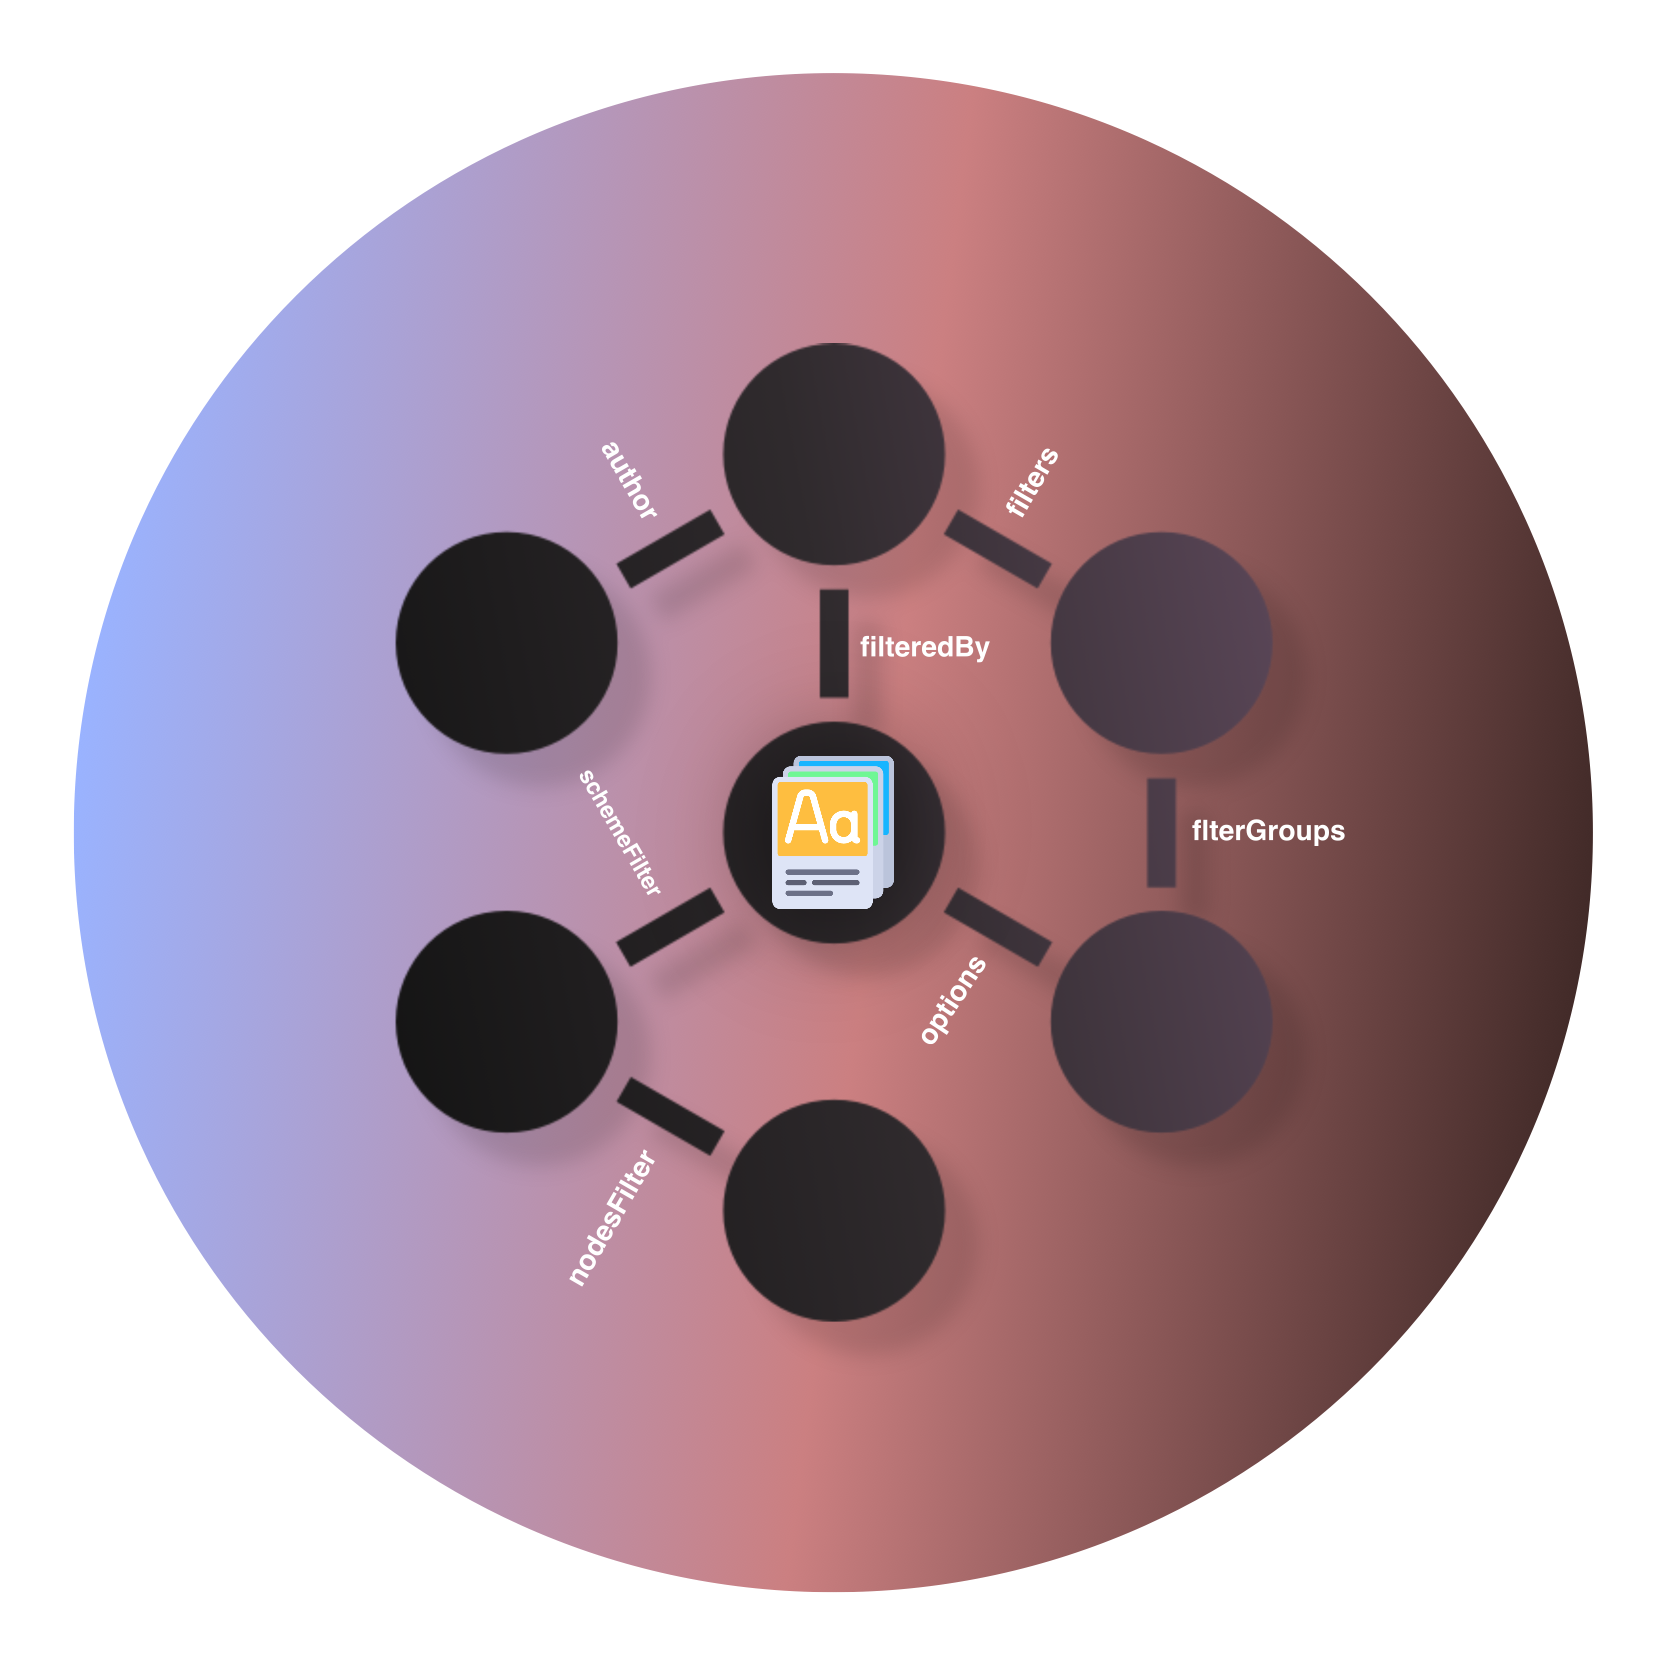
\includegraphics[width=0.4\linewidth]{lpa_ontology_logo.png}}
\caption{Official \lpas{} Ontology logo designed by author.}
\label{fig:lpa_ontology_logo}
\end{figure}

The ontology itself was implemented using a set of open-source tools that will be described in the first part of this section. 

\subsection{Preliminaries}

Two open-source frameworks were used to implement and publish the \lpas{} ontology:
\begin{itemize}
    \item \texttt{Protégé}, is an open-source ontology editing framework developed at Stanford University and written in Java programming language \cite{protege}. It provides an intuitive graphical user interface for defining and developing ontologies. The version of the software used at the moment of implementing the ontology is \texttt{v5.5.0}.
    \item \texttt{Ontoology}, is an open-source software solution for collaborative development of ontologies on GitHub \cite{ontoology}. However, in the scope of implementing \lpas{} ontology, it was mainly chosen for its additional features, such as an ability to publish ontologies under permanent \texttt{w3id.org} URL, an ability to host the ontology as a static HTML webpage under GitHub Pages. 
\end{itemize}

\begin{figure}[h]
\centering
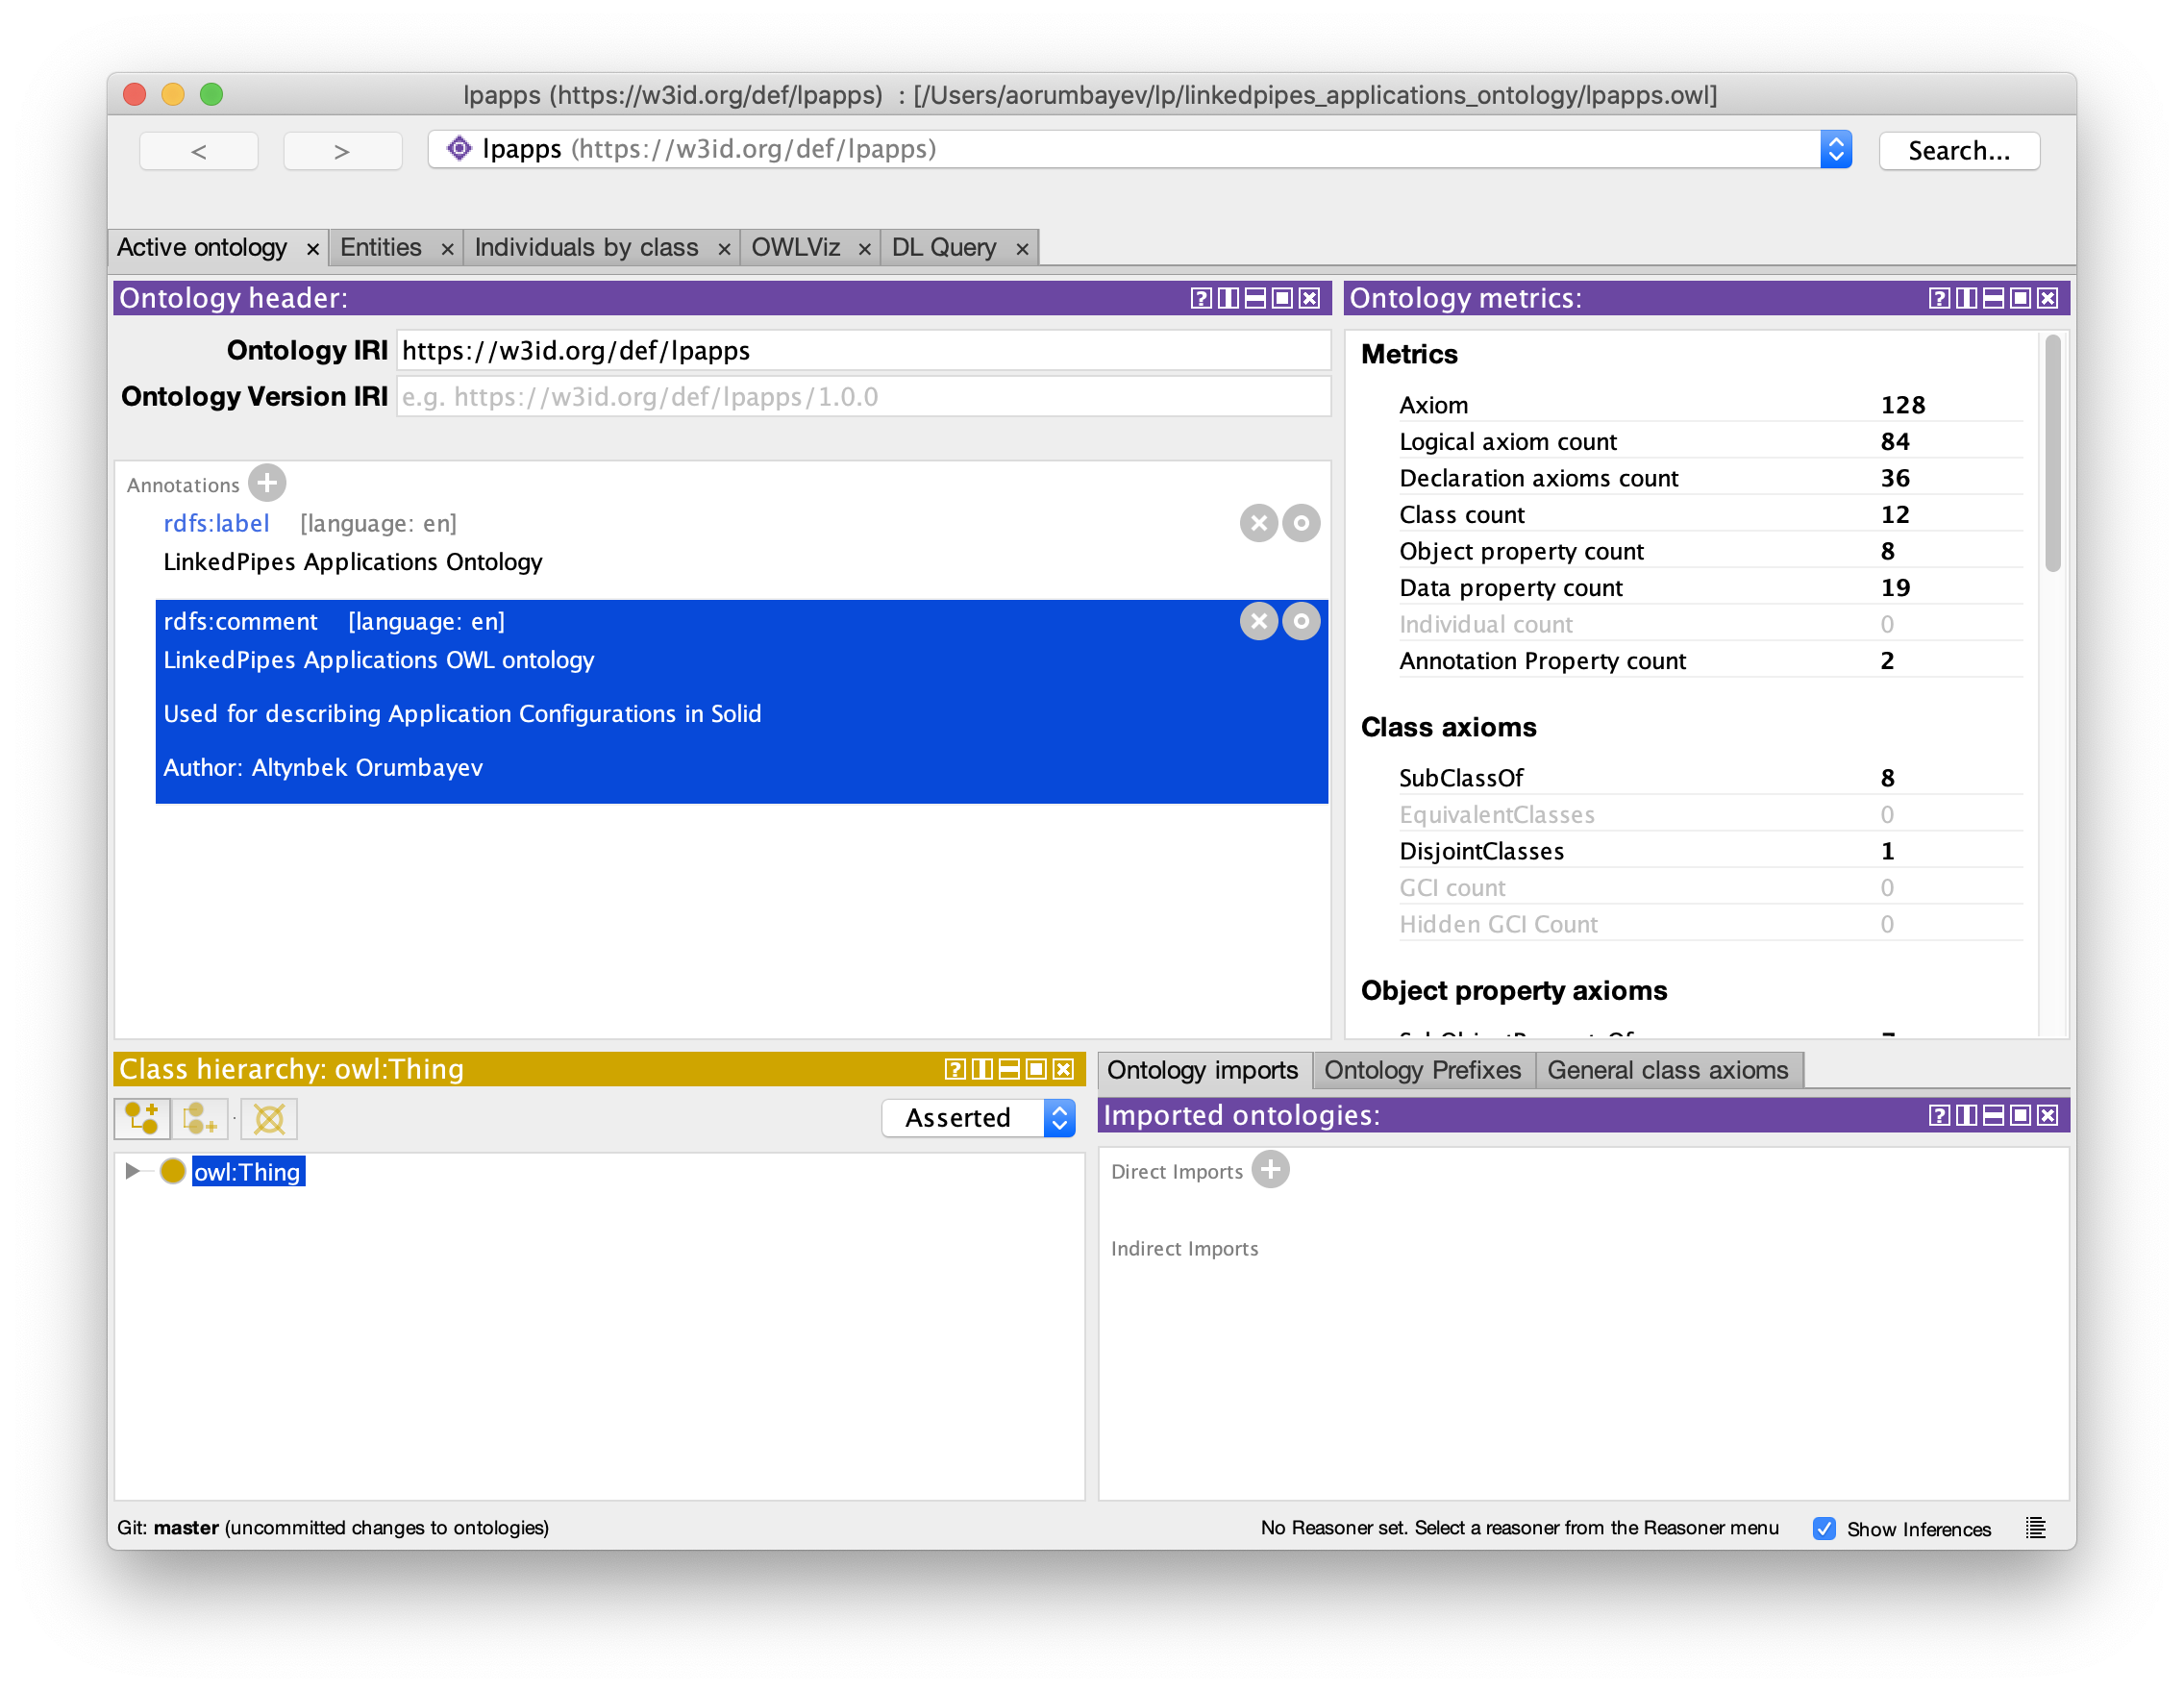
\includegraphics[width=12cm]{misc_ontology_visualizer.png}
\caption{Example UI of \texttt{Protégé} ontology editor at \textit{Active Ontology} tab.}
\label{fig:misc_ontology_visualizer}
\end{figure}

\subsection{Using \texttt{Protégé}}

After defining the main entities and designing the hierarchical structure of the ontology in \autoref{ssec:lpas_application_ontology_arch}, the ontology was implemented using \texttt{Protégé} ontology editor. The editor allows defining the ontology entities by specifying them under:
\begin{itemize}
    \item \textit{Classes}, tab represents the \textit{asserted} and \textit{inferred} class hierarchies as a tree, where each node represents a particular class. The \textit{asserted} class view is a default and primary navigation device for browsing class hierarchies in \textit{Protégé}, the \textit{inferred} classes view on the other hand differs from \textit{asserted} by requiring a reasoner to be setup to render the complete hierarchy view. If no reasoner is provided the \textit{inferred} classes view will be empty.
    \item \textit{Object properties} tab,  represents the graphical user interface to create and define relations between instances of the classes. The view under that tab is similar to the \textit{Classes} tab, the properties are represented as a tree with nodes identifying individual object property. For instance, each \textit{VisualizerConfiguration} can be filtered by a \textit{FilteredConfiguration}, this relation can be expressed by defining an object property calls \textit{filteredBy}.
    \item \textit{Data properties} tab, represents the graphical user to create and define relations between instances of classes and RDF literals or datatypes. For instance, a \textit{VisualizerConfiguration} class has a \textit{backgroundColor} data property which is a \textit{String} datatype. 
\end{itemize}

The resulting ontology created in \texttt{Protégé} was represented as an OWL which is a format for Web Ontology Language described earlier in \autoref{sssec:using_web_ontology_language}. The following subsection will describe the process of publishing the ontology using the \textit{Ontoology} software. 

\subsection{Using \textit{Ontoology}}

The \textit{Ontoology} itself is an open-source project that can be instantiated and configured manually. It is, however, also available as a standalone running instance \footnote{\url{http://ontoology.linkeddata.es}}. The publishing of the \lpas{} Ontology was done using the available instance instead of manually configuring one, this significantly reduced the development time needed to publish and host the vocabulary to be used in \lpa{} frontend.

The initial configuration or startup guide to \textit{Ontology} consist of the following steps: 
\begin{enumerate}
    \item \textit{Setup a GitHub repository}, an exported OWL file from \texttt{Protégé} was hosted on a regular public GitHub repository \footnote{\url{https://github.com/aorumbayev/linkedpipes_applications_ontology}} and placed at the root.
    \item \textit{Add repository to Ontoology}, add the repository by name into Ontology, and press \textit{Watch this repo} button. This is pretty much the last step involving any manual work. The following steps are all invoked in an automated fashion, demonstrating the full list of benefits provided by this software.
    \item \textit{Merge initial PR from Ontoology}, once the repository is connected, an automated PR will be opened that will contain a following list of elements:
    \begin{enumerate}
        \item Diagrams, a folder with pre-generated class hierarchy visualizations of the ontology.
        \item Documentation, an automatically generated ontology documentation hosted on GitHub Pages on the same repository, and available at \textit{w3id.org} permanent URL redirecting users to GitHub Pages.
        \item Evaluation report, \textit{Ontoology} generates a report that checks various aspects of the implementation of the ontology, providing hints when, for instance, some parts in the description of an entity is missing.
        \item JSON-LD, an original OWL the file is automatically converted into a JSON-LD file.  
    \end{enumerate}
\end{enumerate}

\begin{figure}[h]
\centering
\fcolorbox{black}{white}{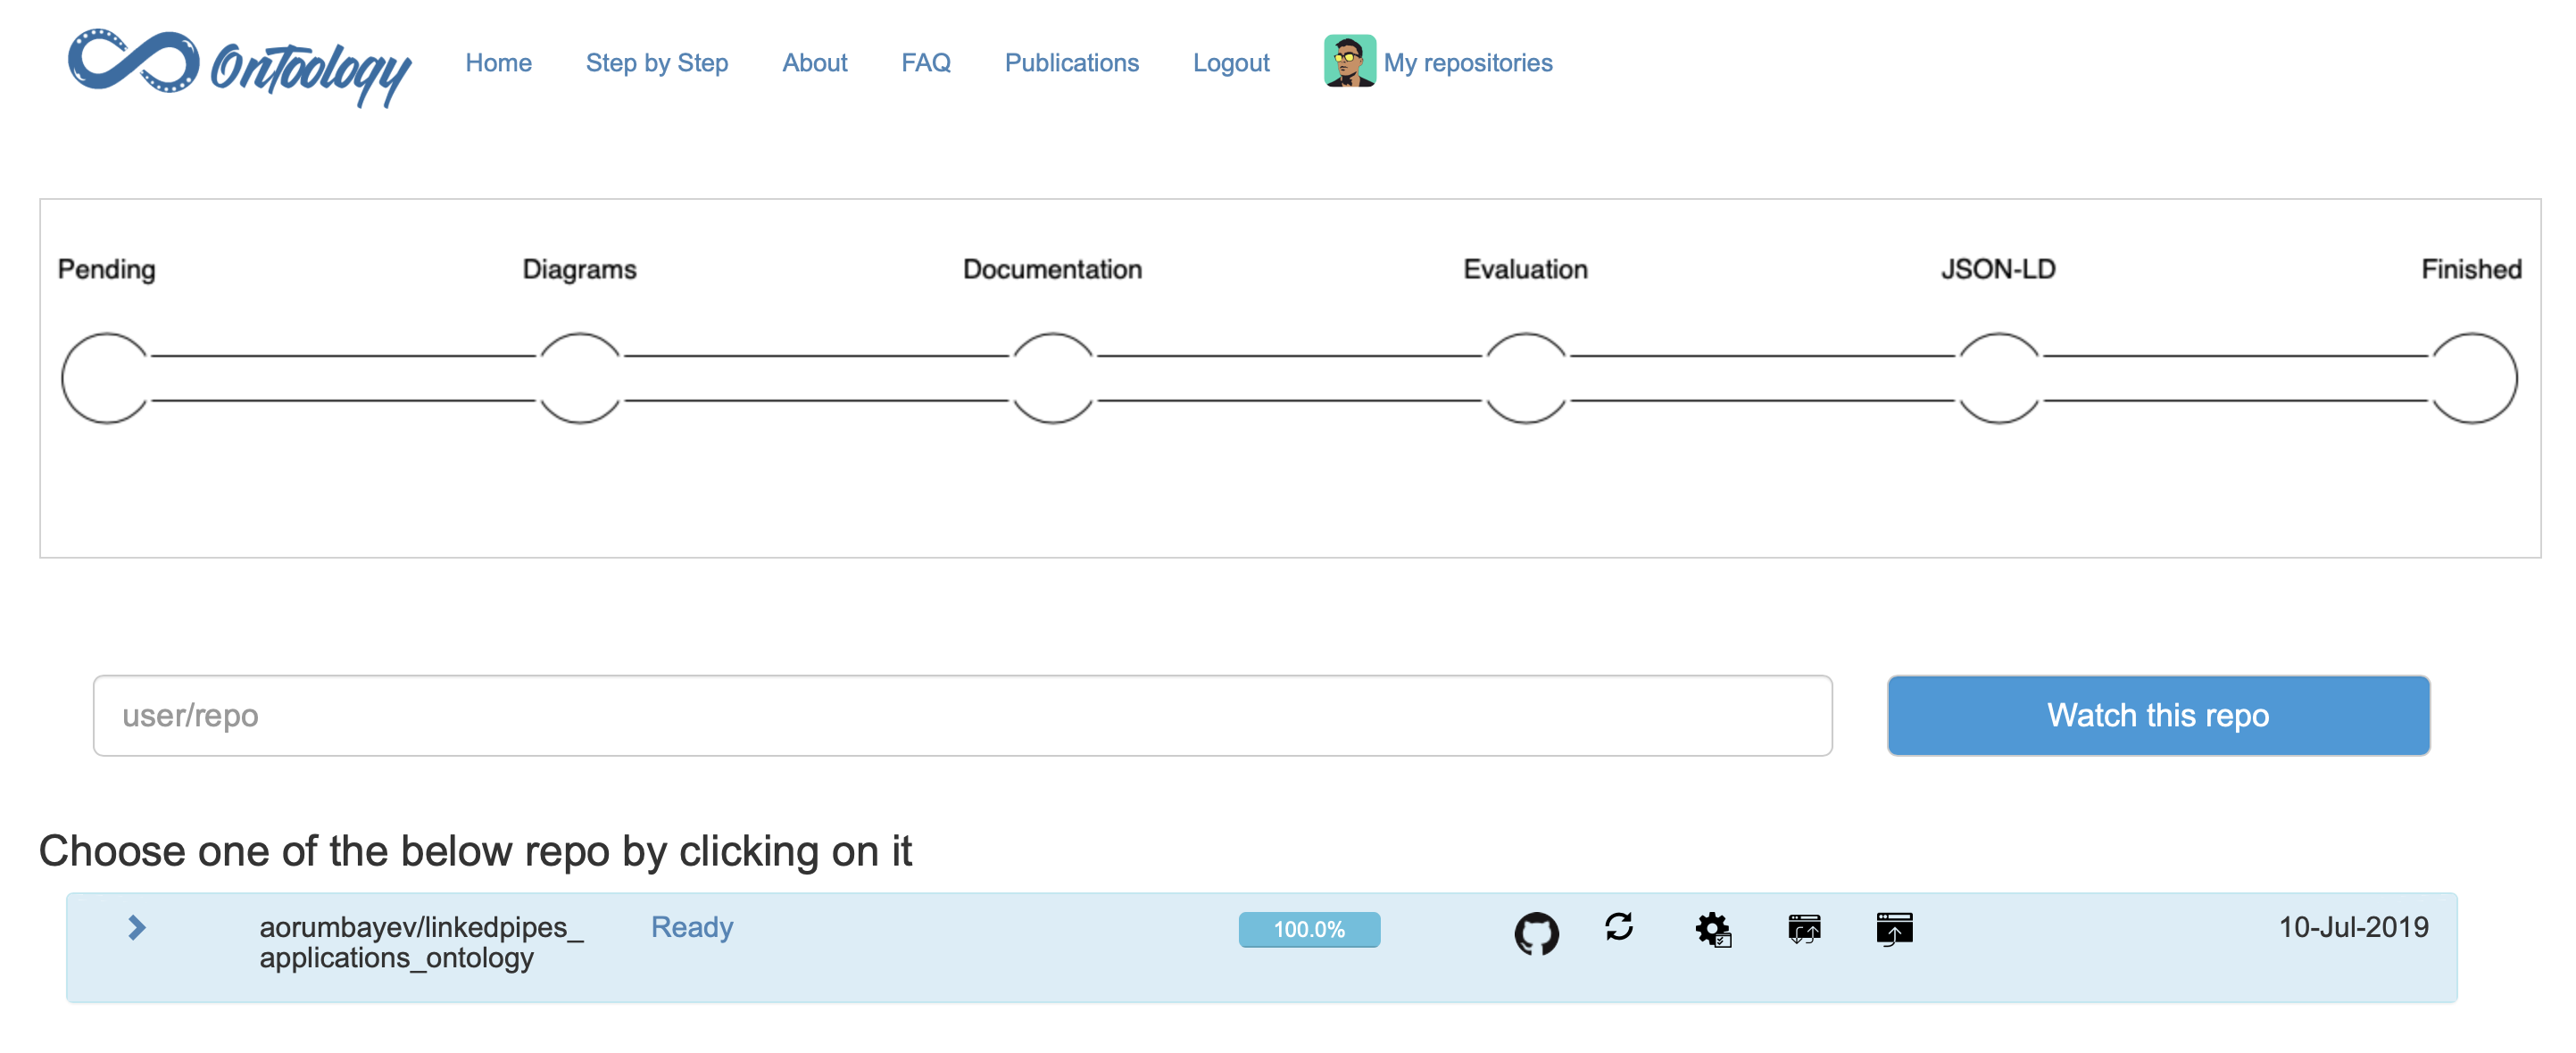
\includegraphics[width=0.8\linewidth]{misc_ontoology_ui.png}}
\caption{UI of Ontoology displaying the processed repository with \lpas{} Ontology.}
\label{fig:misc_ontoology_ui}
\end{figure}

To sum up, the \lpas{} ontology was implemented using two open-source frameworks called \texttt{Protégé} and \texttt{Ontoology}. The first tool was used as an editor to implement the ontology designed in \autoref{ssec:lpas_application_ontology_arch}. The second tool was used to publish and host applications. The detailed documentation will be mentioned in \autoref{chap:num_8} and is also available at \url{http://w3id.org/def/lpapps}. 

\section{Storage Frontend}
\label{sssec:lpas_storage_frontend_implementation}

The following section will continue the \autoref{ssec:lpas_storage_component_design} by providing the details on implementation of individual components interacting with \solid{} POD. 

\subsection{Preliminaries}
\label{sssec:preliminaries_storage_frontend}

To simplify the understanding of this section, it is important to recap the conventions and specifics of \lpa{} frontend implementation by providing some extended details, as they were strictly taken into consideration while developing \lpas{} components inside the \lpa{} frontend codebase.

As mentioned earlier in \autoref{sssec:lpa_preliminaries_component_overview}, the frontend provides a way for the user to interact with the \lpa{}. As demonstrated on the \autoref{fig:lpa_frontend_architecture}, the frontend uses Redux and React as a primary framework for building the components and managing states.

\begin{figure}[h]
\centering
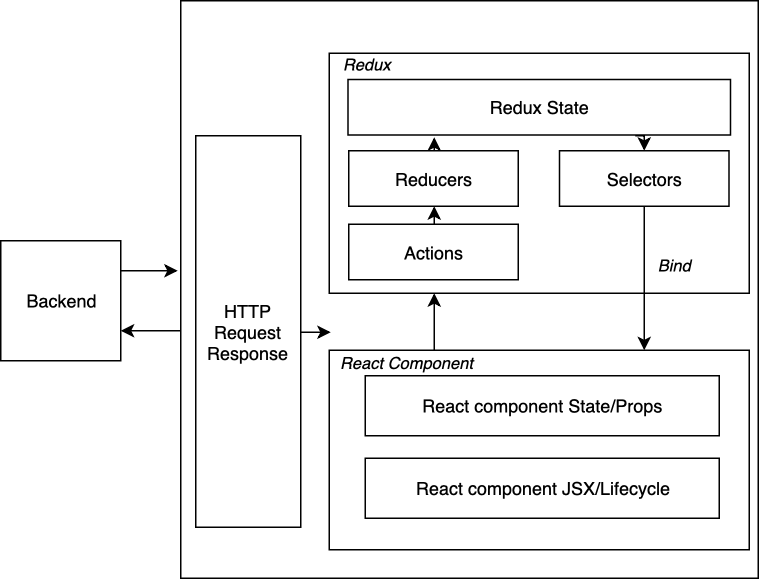
\includegraphics[width=12cm]{lpa_frontend_architecture.png}
\caption{General architecture of Redux store and React components within \emph{frontend}}
\label{fig:lpa_frontend_architecture}
\end{figure}

The main entities displayed on \ref{fig:lpa_frontend_architecture} can be described as follows:

\begin{itemize}
    \item \textit{React Component}, a JavaScript class or function that optionally accepts inputs, i.e., properties(props), and returns a React element that describes how a section of the UI (User Interface) should appear. 
    \item \textit{Redux} represents a container that stores various states of the web application per individual webpage.
        \begin{itemize}
            \item \textit{State}, refers to the single state value that is managed by the store and returned by \texttt{getState()}. It represents the entire state of a Redux application, which is often a deeply nested object.
            \item \textit{Reducer} specifies how the application's state changes in response to actions sent to the store.
            \item \textit{Actions} are payloads of information that send data from your application to your store. They are the only source of information for the store. An action is invoked by sending them to the store using \texttt{store.dispatch()}.
            \item \textit{Selector} is simply any function that accepts the Redux store state (or part of the state) as an argument and returns data that is based on that state.
        \end{itemize}
\end{itemize}

\subsubsection{Frontend code structure}
\label{ssssec:lpa_frontend_code_structure}

The implementation of the \lpa{} frontend is located at the \texttt{src/frontend} path at official \lpa{} repository \footnote{\url{https://github.com/linkedpipes/applications}}  and structured as follows:

\begin{itemize}
    \item \textit{constants} - contains all constants used throughout the frontend component implementation.
    \item \textit{utils} - contains various handy utility classes, variables, and methods.
    \item \textit{ducks} - contains all Redux reducers, actions and selectors. The title \textit{duck} comes from a convention proposed by Erik Rasmussen in \cite{redux_ducks}, it suggests a way to bundle Redux entities into folders that are easier to manage and maintain as they contain reducers, actions and selectors.
    \item \textit{layouts} - contains global setup for various components as well as the specification for the MaterialDesign theme used in the project.
    \item \textit{components} - contains all components with JSX file type, visualizers and various UI elements implementations not related to interactions with \solid{}. The JSX is a syntactic extension for JavaScript that adds ability to combine ES6 syntax with HTML tags.
    \item \textit{containers} - contains complex layouts for specific web-pages of the web app not related to interactions with \solid{}. Each folder is named after individual webpage. 
    \item \textit{storage} - contains all contributions and implementations made within the scope of \lpas{} project. Has a substructure mimicking the global folder structure to improve code maintainability and signify the difference between implementations of \lpa{} and \lpas{}.
    \item \textit{configuration files and entry points}, contains a set of configuration files at the root, such as linter configurations, the file with global Redux store and a file called \textit{AppRouter}, which is the main controller of whole frontend since it manages the user sessions and establishes the socket connections with \lpa{} backend.
\end{itemize}

\subsection{Storage folder structure}
\label{sssec:storage_folder_structure}

As mentioned in \autoref{ssssec:lpa_frontend_code_structure}, let us describe the internals of \textit{storage} folder inside \lpa{} frontend codebase. 

\begin{itemize}
    \item \textit{utils} - contains various handy utility classes, variables, and methods for storage specific React Components.
    \item \textit{ducks} - contains all Redux reducers, actions and selectors for storage specific React Components. 
    \item \textit{models} - contains classes representing \textit{VisualizerConfiguration} and other \lpa{} specific classes that did not have to be split into the \lpas{} package.
    \item \textit{components} - contains all components, visualizers and various UI elements implementations not related to interactions with \solid{}.
    \item \textit{containers} - contains complex layouts for storage specific web-pages. Each folder is named after individual webpage.     
    \item \textit{StorageBackend} - represents a class wrapping various utilities on top of basic \lpas{} storage abstractions. The logic related to fetching the \lpa{} configurations is implemented in this file.
    \item \textit{StorageToolbox} - represents a class wrapping the \textit{StorageBackend} utilities into simple methods to be invoked directly from internal methods of Storage React Components. In other words, it serves as a middleware layer between React Components and low level and generic functionality of \lpas{} package abstractions.
    \item \textit{StorageSparqlClient} - a class containing a single generic method that utilises the \textit{fetch()} function from \textit{AuthenticationManager} to submit \texttt{SPARQL} requests modifying certain parameters of \lpa{} configuration RDF files. 
\end{itemize}

\subsection{Authentication View}
\label{sssec:authentication_view_implementation}

This section continues the architecture and mocks provided in \autoref{ssec:lpas_storage_component_design}, and describes the implementation of the React Component in detail.
To comply with conventions of \lpa{} frontend, the webpage is represented by two separate React Components, one of which is stateful and the other is stateless and manages the views only. The implementation is located at \texttt{src\-/frontend\-/containers\-/AuthenticationPage} path on \lpa{} repository. The folder is named after the webpage and consist of:
\begin{itemize}
    \item \textit{AuthenticationContainer}, a file containing the stateful React Component. In other words, it manages local views specific states as well as global states related to Redux.
    \item \textit{AuthenticationComponent}, a file containing implementation of stateless React Component. In other words it is only responsible for passing the React \textit{props} and rendering simple views.
    \item \textit{SolidProviderComponent}, a file located in a sub-folder called \textit{children}. Component renders the drop-down menu that allows users to pick specific provi\-der from a list of supported \solid{} providers.
\end{itemize}

\begin{listing}[H]    
\begin{minted}[breaklines,frame=single,framerule=1pt,bgcolor=LightGray]{javascript}
const mapStateToProps = state => {
  return {
    webId: state.user.webId
  };
};

export const AuthorizationContainer = connect(mapStateToProps)(Authorization);
\end{minted}
\caption{An example of mapping Redux state to a props of React Container} 
\label{lst:map_state_to_props_example}
\end{listing}

Following that pattern, the \textit{render()} function of \textit{AuthenticationContainer} expects an instance of \textit{AuthenticationComponent} while passing both internal and Redux state as props to it. The global structure of all Redux states in \lpa{} is to specific to be described within the scope of the \lpas{} project, however an examples of states relevant to Authentication View are going to be provided. For instance, the code example at \autoref{lst:map_state_to_props_example} demonstrates a typical example of an operation that maps the Redux states to \textit{props} of a React Component, in this case we are mapping the global \textit{webID} value that is used by React Router to identify whether user is authenticated and can render the dashboard or should be redirected back to the screen. As it was mentioned earlier in \autoref{ssssec:lpa_frontend_code_structure} and \autoref{sssec:authentication_manager_implementation}, the \textit{AppRouter} is one of the main entry points to the frontend web app, and it directly utilizes both \textit{AuthenticationManager} abstraction from Authentication React component. An example code on \autoref{lst:track_session_example} demonstrates a code snippet from \textit{AppRouter} that is invoked every time user session is being authenticated or user is logging out.

\begin{listing}[H]    
\begin{minted}[breaklines,frame=single,framerule=1pt,bgcolor=LightGray]{javascript}
AuthenticationManager.trackSession(session => {
  if (session) {
     handleSetUserWebId(session.webId);

     self.startSocketListeners();
     ...
  }
})
\end{minted}
\caption{An example of \textit{trackSession()} callback listening for changes in authentication state} 
\label{lst:track_session_example}
\end{listing}

The User Interface strictly follows initial mock design demonstrated at \autoref{fig:lpas_authenticate_mock}. User has an ability to perform authentication either by choosing an individual \solid{} provider or use a supply his WebID directly if his \solid{} provider is not available in the list of default providers. At the moment of writing this part, the project provides support for \texttt{inrupt.net} \footnote{\url{https://inrupt.net}}, \texttt{solid.community} \footnote{\url{https://solid.community}} and self-hosted provider made specifically for LinkedPipes available at \textit{lpapps.co} \footnote{\url{https://lpapps.co:8443}}. After performing the authentication use is redirected into the Dashboard webpage of \lpa{} frontend.

\subsubsection{Overview of states and methods}

As general details on the structure of the implementation are defined now, let us dive deeper into the description of main states and functions of Authentication View components. As \textit{AuthenticationComponent} is a stateless React component, it is sufficient to provide definitions for states and methods in \textit{AuthenticationContainer} as this represents the main functionality of the whole webpage. The states can be described as follows:
\begin{itemize}
    \item \textit{webIdFieldValue}, a \texttt{string} value holding input at the \textit{textfield} for supplying WebID value.
    \item \textit{withWebIdStatus}, a \texttt{boolean} value representing the current input state and whether is chosen to use available providers or entered his WebID manually.
    \item \textit{session}, an \texttt{object} representing current session returned from \textit{AuthenticationManager} abstraction.
    \item \textit{providerTitle}, a \texttt{string} value holding the title of selected provider. This is needed to be supplied into \textit{login()} method of \textit{AuthenticationManager} abstraction that invokes the \texttt{solid-auth-client} library.  
\end{itemize}

The set of methods inside the \textit{AuthenticationComponent} class can be described as follows:
\begin{itemize}
    \item \textit{handleProviderChange()} a methods that is passed as a \texttt{prop} to \textit{AuthenticationComponent}, and invoked every time user selects or update his selection of default providers.
    \item \textit{handleSignIn} a method that is invoked when is pressing the \textit{Authenticate} button, this redirects a call to \textit{AuthenticationManager} abstraction that initiates the sequence flow described at \autoref{fig:lps_authentication_sequence_diagram}.
    \item \textit{handleWebIdFieldChange} a method invoked when user inputs or modifies the input at the \textit{textfield} used for WebID.
    \item \textit{isWebIdValid} a method that uses \textit{regex} to validate whether provided WebID is in valid format.
    \item \textit{onSetWithWebId} a method invoked when the \textit{withWebIdStatus} status is being changed.  
\end{itemize}

The final rendered UI of this implementation will be provided in the of this chapter under \autoref{ssec:overview_of_implemented_requirements}, where a detailed overview of a final implementation satisfying each of the original \lpa{} requirements are provided.

\subsection{Storage Dashboard}
\label{sssec:storage_dashboard_implementation}

The Storage Dashboard webpage described at \autoref{sssec:architecture_storage_dashboard} was a challenging component to implement. To simplify the understanding of the structure in which components and containers are invoked, the \autoref{fig:storage_dashboard_implementation_diagram} is provided. The components demonstrated on diagram follow the usual pattern of splitting React Components into stateful and stateless and can be described as follows:
\begin{itemize}
    \item \textit{StoragePageController} is a root React component that wraps both individual and shared application views. It stores states representing the tab index and depending on the selected index it switches the components to be rendered in \textit{render()} function.
    \item \textit{StorageAppsBrowser*}, both container and component represent a view that fetches and displays \lpa{} configurations. The stateless part relies on the \textit{Grid} layout system from \texttt{MaterialUI} framework.
    \item \textit{StorageSharedAppsBrowser*}, both container and component represent a view that fetches and displays \lpa{} configurations that were shared with the User. The stateless part relies on the \textit{Grid} layout system from \texttt{MaterialUI} framework.
    \item \textit{StorageAppsBrowserCardComponent} is a child component that represents a reusable card representing an individual \lpa{} configuration in a grid of cards.
\end{itemize}

The user interface is inspired by the mock at \autoref{fig:lpas_ui_dashboard_mock}. However, it is more refined and optimized to fit the general style of \lpa{} frontend. Similar to the Authentication view, the final rendered UI of this implementation will be provided at the end of this chapter under \autoref{ssec:overview_of_implemented_requirements}.

\begin{figure}[h]
\centering
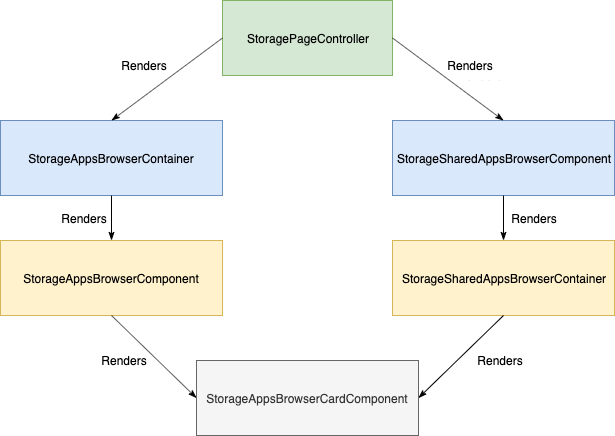
\includegraphics[width=10cm]{storage_dashboard_implementation_diagram.png}
\caption{Diagram representing the chain of \textit{render()} method invocations among components representing Storage Dashboard.}
\label{fig:storage_dashboard_implementation_diagram}
\end{figure}

\subsubsection{Overview of main functionality}

In contrast with Authentication View, the structure of sub-components is rather complex to describe in detail. Therefore a set of primary states and methods responsible for the core functionality of the webpage will be described instead.

In general both \textit{StorageAppsBrowser*} and \textit{StorageSharedAppsBrowser*} components and containers share similar states and functions the only difference is the way stored \lpa{} configurations are fetched. The fetching itself is done by invoking the corresponding methods called \textit{getAppConfigurationsMetadata()} and \textit{getSharedApplicationsMetadata()} methods from \textit{StorageToolbox} class. In general, the \textit{StorageToolbox} invokes lower-level wrappers in \textit{StorageBackend} that utilize the \texttt{rdflib} library from \lpas{} package and converts the RDF resource representing the \lpa{} configuration into a JavaScript object that is processed by \textit{StorageAppsBrowserCardComponent} view.

\subsection{Storage Control Panel}
\label{sssec:storage_control_panel_implementation}

The Storage Control Panel is rather a simple set of React Components that heavily rely on \textit{FileManager} abstraction from \lpas{} package. As initially described in \autoref{sssec:architecture_storage_control_panel}, the functionality should provide user options to perform basic operations with the root folder for all \lpa{} configurations in his \solid{} POD. Those operations include changing the title of the root folder, moving within the pod, or copying within the pod. The implementation consist of the following classes:
\begin{itemize}
    \item \textit{StorageAccessControlDialog} is a stateful React Component based on \textit{Dialog} Component from \textit{Material UI} framework. Due to simplicity of the elements to be rendered, it did not require splitting into stateful and stateless components.
    \item \textit{SettingsPageComponent} is a stateless React Component that renders the simple label with the current path to the root storage folder in \textit{Solid} and a simple button to change it by invoking the \textit{StorageAccessControlDialog}.
    \item \textit{SettingsPageContainer} is a stateful React Component that serves to connect the \textit{StorageAccessControlDialog} and \textit{SettingsPageComponent}.
\end{itemize}

\subsubsection{Overview of main functionality}

In general, the main functionality is located in the \textit{StorageAccessControlDialog} class, it strictly follows the mock at \autoref{fig:lpas_change_folder_mock} and can be described as follows:
\begin{itemize}
    \item \textit{handleFolderConfirm()} a method invoked when user clicks on \textit{Update} button. The component then invokes the \textit{StorageToolbox} class that communicates with \textit{FileManager} abstraction in \lpas{} package. For more detailed description of how \lpas{} package performs the \texttt{CRUD} operations on resources in \solid{} PODs refer back to \autoref{chap:num_4}.
    \item \textit{handleFolderCopy()} a method invoked when user clicks on \textit{Copy} button. The rest is similar to \textit{handleFolderConfirm()} where \textit{StorageToolbox} is invoked and it communicates with \textit{FileManager} abstraction in \lpas{} package. 
    \item \textit{handleFolderMove()} a method invoked when user clicks on \textit{Move} button. The proceeding invocation chain is identical to methods before.
\end{itemize}

The final rendered UI of this implementation will be provided in \autoref{ssec:overview_of_implemented_requirements}, demonstrating the \textit{StorageAccessControlDialog}, \textit{SettingsPageComponent} and \textit{SettingsPageContainer}.

\section{Implemented functional requirements}
\label{ssec:overview_of_implemented_requirements}

This section will iterate over the requirements from \lpa{} stated in \autoref{chap:num_3}, and demonstrate how each of the functional requirement was implemented by classes and abstractions described in previous sections of this chapter. For requirements that directly involved the implementation of React components, detailed renders of final User Interfaces will be provided. It is important to note that this section provides the implementation overview of all stated functional requirements defined in \autoref{ssec:functional_requirements}.

\subsection{User Authentication}

To recap the User Authentication functional requirement, the user of the platform should be able to register an account in the application, log in, and log out. To fulfill the requirement, the Authentication View component described at \autoref{chap:num_1} was implemented. The final render on \autoref{fig:lpa_login_webpage} provides an intuitive User Interface that allows authentication by selecting a default \solid{} provider, as demonstrated on \autoref{fig:lpa_login_webpage_dropdown} or by specifying the WebID for authentication directly. The \textit{Learn more about WebID, and SOLID} button serves as a guide for users new to \solid{}, clicking the button will get them redirected to the official \texttt{inrupt} website. 

\begin{figure}[hbt]
\minipage{0.5\textwidth}
  \fcolorbox{black}{white}{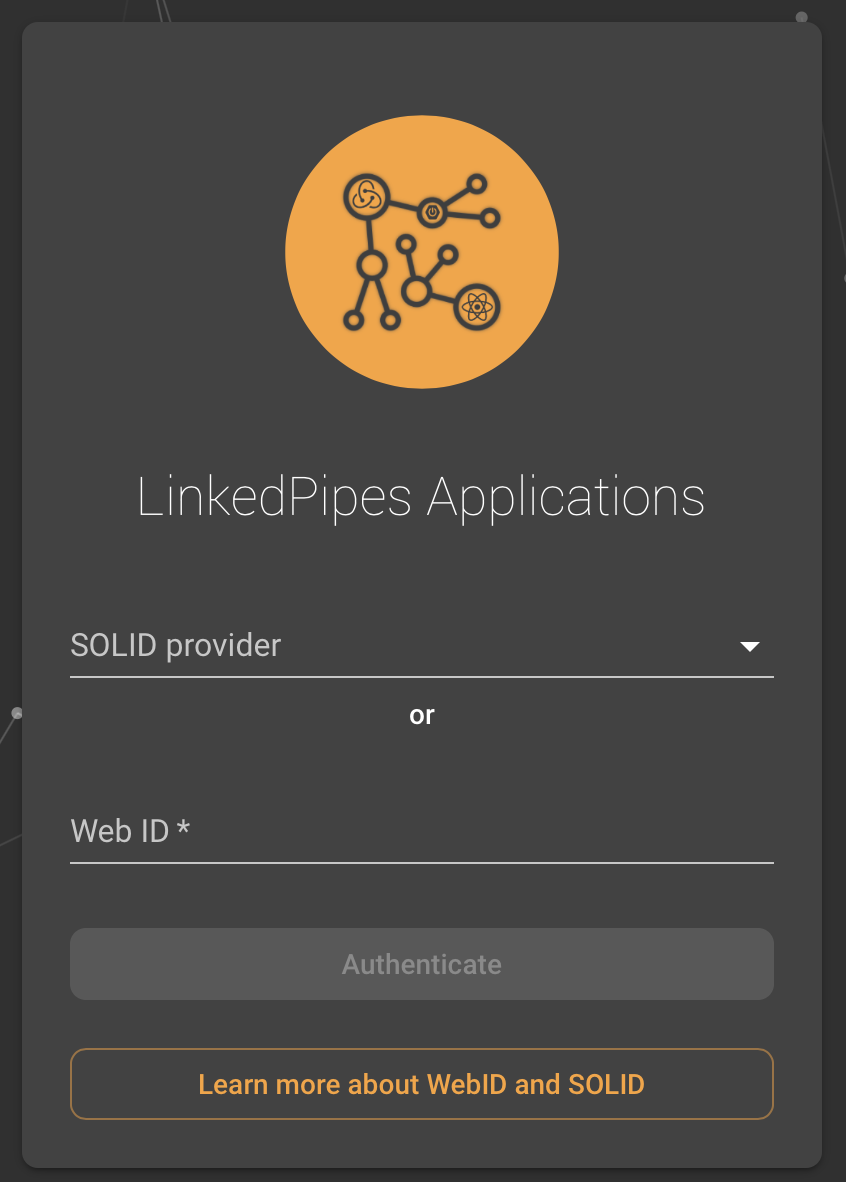
\includegraphics[width=0.8\linewidth]{lpa_login_webpage.png}}
  \caption{The final render of an Authentication View webpage}
  \label{fig:lpa_login_webpage}
\endminipage\hfill
\minipage{0.5\textwidth}
  \fcolorbox{black}{white}{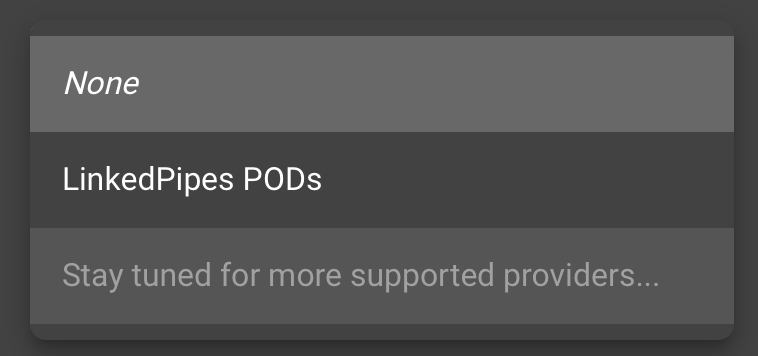
\includegraphics[width=0.8\linewidth]{lpa_login_webpage_dropdown.png}}
  \caption{And example of the \textit{providers} dropdown in expanded state.}
  \label{fig:lpa_login_webpage_dropdown}
\endminipage\hfill
\end{figure}

After user provides the authentication inputs and clicks on \textit{Authenticate} button, the default \solid{} server authentication popup will appear as demonstrated on \autoref{fig:solid_login_webpage} and \autoref{fig:solid_register_webpage}. Depending on whether user has a WebID and a \solid{} POD or if user selected the authentication option using default providers he will be given an option to either \textit{Login} or \textit{Register} on specified \solid{} server. 

\begin{figure}[hbt]
\minipage{0.6\textwidth}
  \fcolorbox{black}{white}{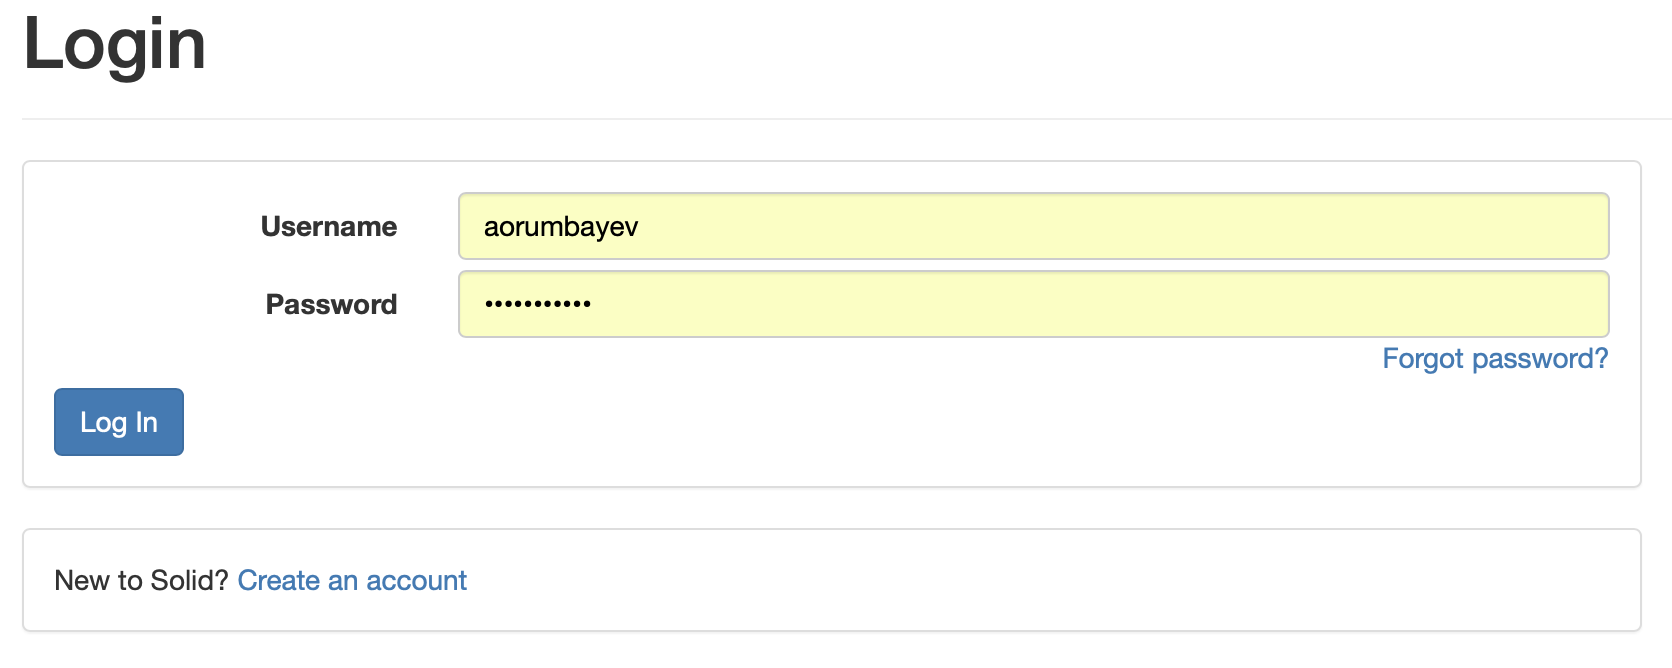
\includegraphics[width=0.8\linewidth]{solid_login_webpage.png}}
  \caption{Example of a login popup provided by \solid{} server.}
  \label{fig:solid_login_webpage}
\endminipage\hfill
\minipage{0.3\textwidth}
  \fcolorbox{black}{white}{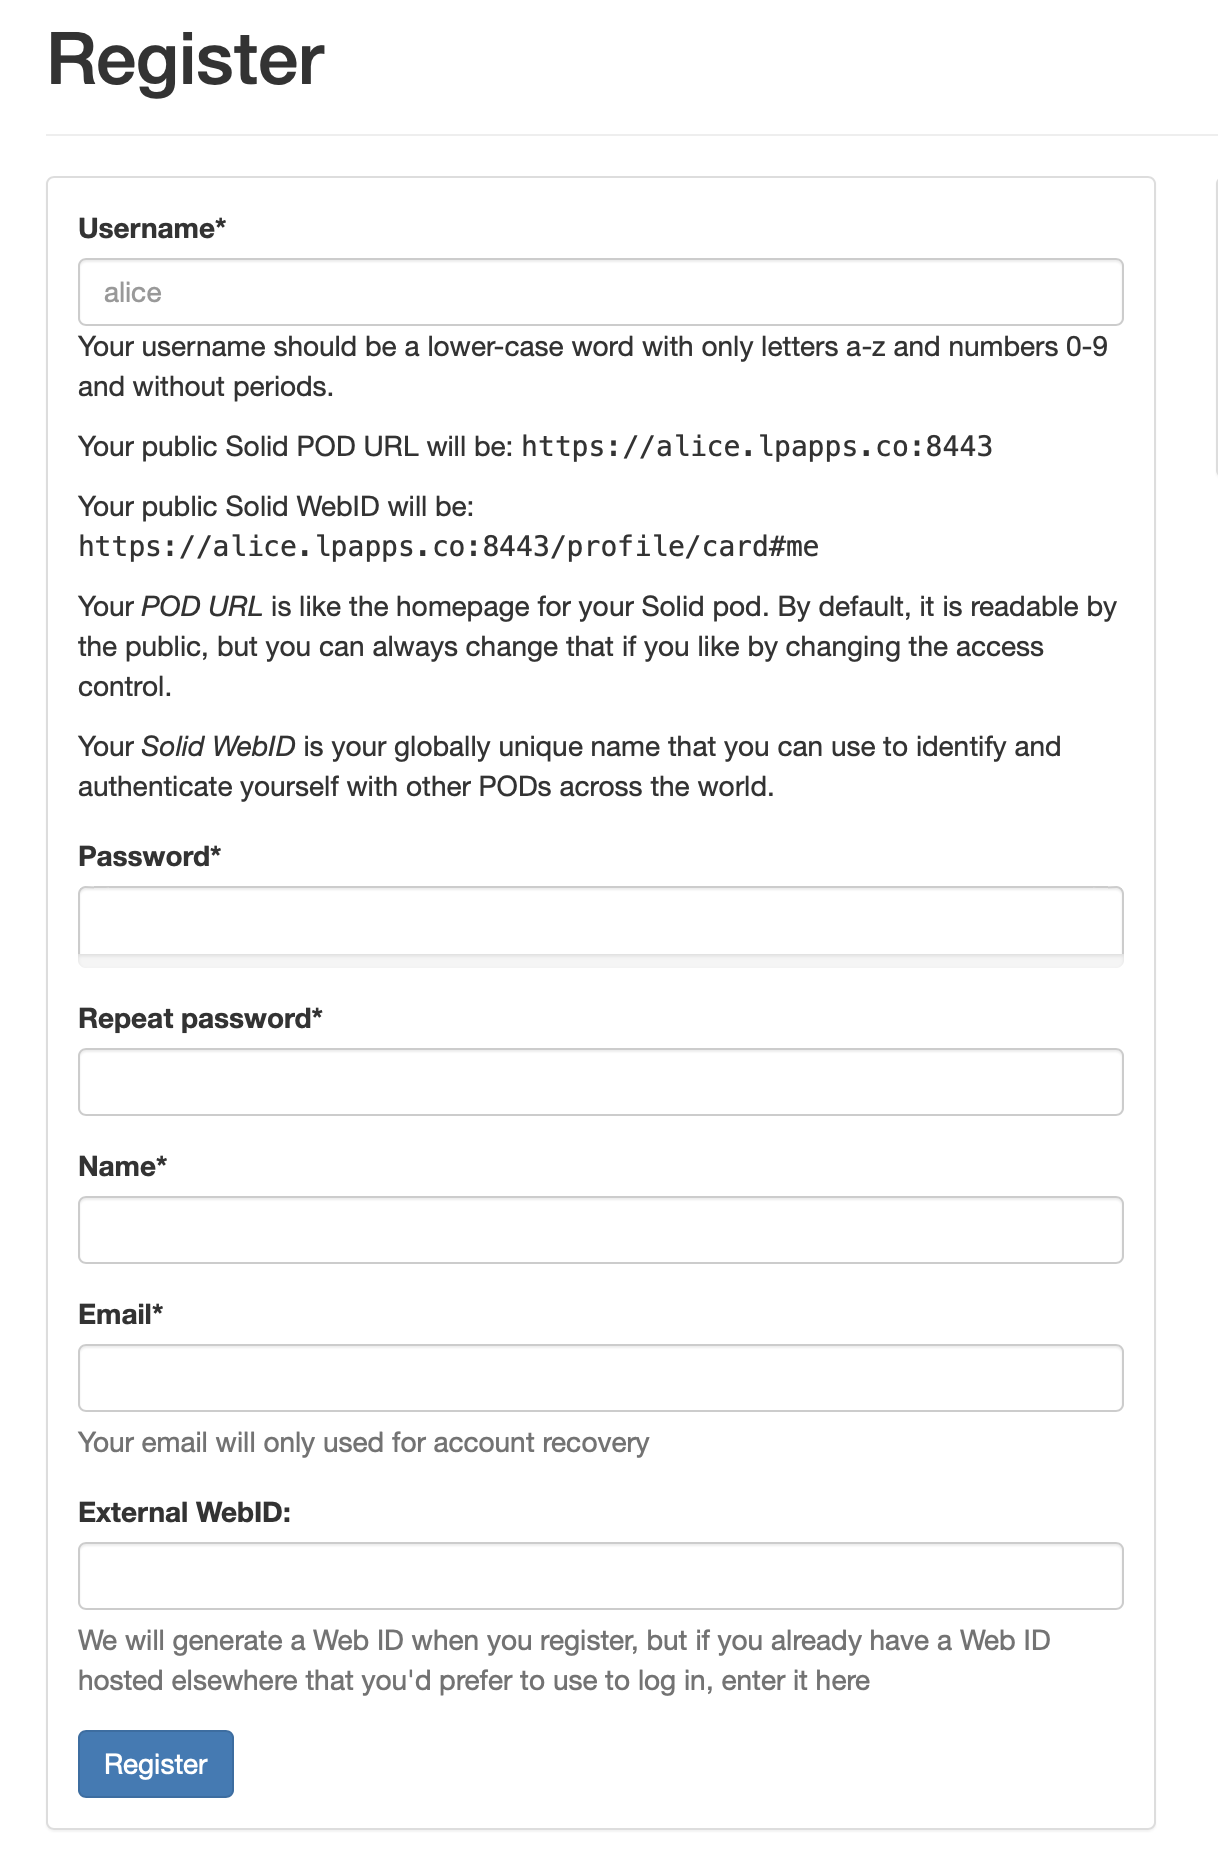
\includegraphics[width=0.8\linewidth]{solid_register_webpage.png}}
  \caption{Example of a register popup provided by \solid{} server}
  \label{fig:solid_register_webpage}
\endminipage\hfill
\end{figure}

The \textit{logout} functionality is available under several components in \lpa{}. Those can be described as follows:
\begin{itemize}
    \item \textit{User Profile Page}, this page is located under settings tab in \lpa{} platform. The intent is to provide the information about the current user name and his WebID under which the authentication was performed. It also provides buttons to either \textit{Reset Password} or \textit{Logout} from the platform.
    \item \textit{Logout toolbar item}, this is a toolbar element always available in the top right corner of the platform. Clicking on the button invokes the \textit{logout}, and the user is redirected back to the Authentication View webpage.
\end{itemize}

\begin{figure}[hbt]
\minipage{0.5\textwidth}
  \fcolorbox{black}{white}{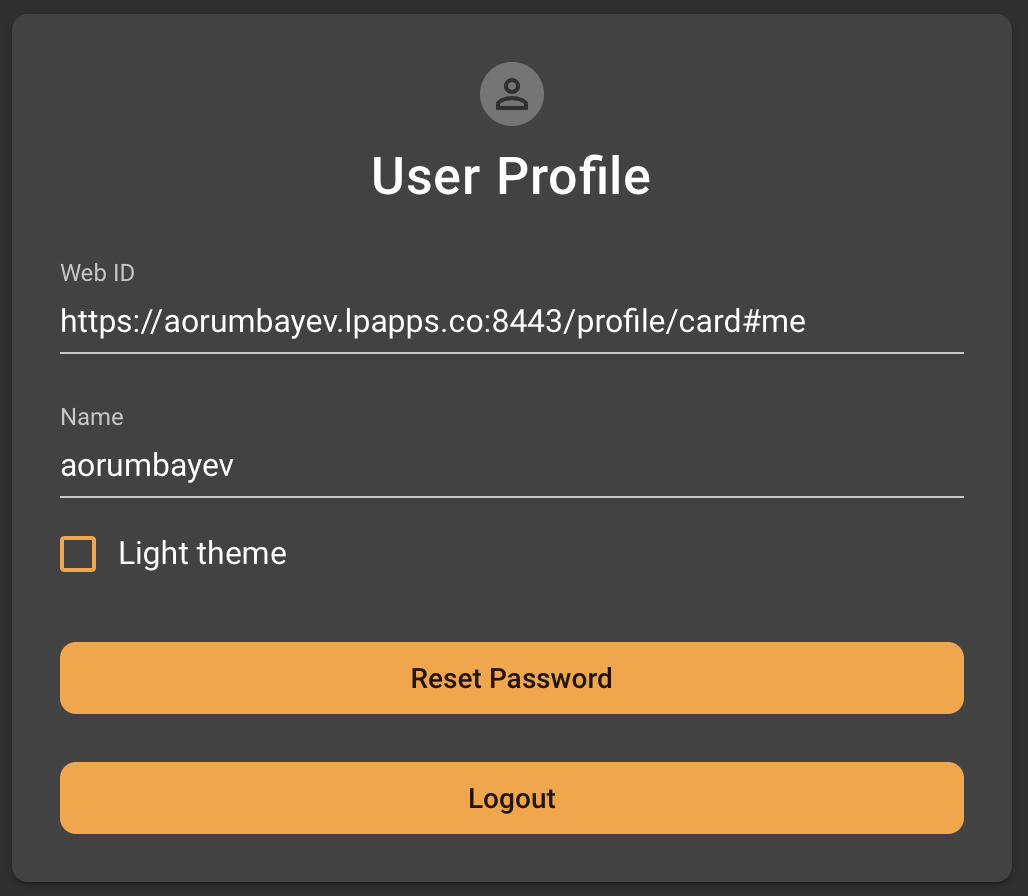
\includegraphics[width=0.8\linewidth]{lpa_user_profile_page.png}}
  \caption{The User Profile webpage with options to reset or logout from \solid{} provider.}
  \label{fig:solid_user_profile_login_webpage}
\endminipage\hfill
\minipage{0.4\textwidth}
  \fcolorbox{black}{white}{
\includegraphics[width=0.8\linewidth]{lpa_user_profile_page_logout.png}}
  \caption{The global control toolbar of \lpa{} platform. The logout button allows to quickly logout from authenticated \solid{} provider.}
  \label{fig:solid_toolbar_logout}
\endminipage\hfill
\end{figure}

\subsection{Create, Store and Publish Application}

The Create and Publish Application requirements are one of the core requirements that are both applicable to \lpas{} and \lpa{} frontend itself. The separation of code contributions to both \lpa{} and \lpas{} was a challenging task. From the standpoint of \lpas{}, an application is created when its configuration is stored as an RDF resource inside \solid{} POD. Having a stored configuration also implies that the application described by this configuration is published because the URI to configuration inside the POD is publicly available by default. In other words, storing creation and publishing of the application are closely related requirements that are easier to cover at once. The section will also focus on the parts of these functional requirements that directly related to interactions with \solid{} server. Additionally, It is important to mention that there is no actual application being stored in the \solid{} pod, the app itself is a React Component that is re-rendered from scratch based on the \lpa{} configuration that is loaded from the storage. 

The \lpa{} platform has a process called \textit{Application data preparation workflow}. It consists of four steps during which a user of the platform provides data sources to visualize, and if successful, the \lpa{} redirects him to a \textit{Create Application} webpage. At this point, the platform assembles a visualizer configuration object in memory until the user provides a title for his application and decides to publish it. The diagram on \autoref{chap:num_1} demonstrates the user interface component on \textit{Create Application} that consist of a text field and two buttons:
\begin{itemize}
    \item \textit{Publish} a button that invokes a chain of methods that parse the prepared visualizer object into TTL and uploads the file into his \solid{} POD.
    \item \textit{Embed} a button invoking the same process of storing and publishing an application but additionally displays a dialog popup to quickly generate the HTML \texttt{iframe} to incorporate the visualizer into a webpage.
\end{itemize}

\begin{figure}[h]
\centering
\fcolorbox{black}{white}{
\includegraphics[width=0.8\linewidth]{lpa_create_application_page.png}}
\caption{A part of \textit{Create Application} page that invokes creation and publishing of an application.}
\label{fig:create_app_implementation_diagram}
\end{figure}

A method source code demonstrated on \autoref{lst:save_app_to_solid_chunk} is invoked by \textit{CreateVisualizerPage} and its underlying sub components. As the first step, it simply checks whether the \texttt{webId} is provided. Afterwards, the \texttt{application\-Configuration\-Object} is assembled which is a JavaScript \textit{object} with fields corresponding to \lpas{} Ontology. When passed into \textit{StorageBackend} the object is parsed into an \texttt{rdflib} graph, serialized into TTL and uploaded into \solid{} using \lpas{} package.

\begin{listing}[H]    
\begin{minted}[breaklines,frame=single,framerule=1pt,bgcolor=LightGray]{javascript}
async saveAppToSolid(
  applicationConfiguration,
  filtersConfiguration,
  webId,
  appFolder
): Promise<ApplicationMetadata> {
  if (!webId) {
    Log.error('No webID available', 'StorageToolbox');
    return;
  }

  const applicationConfigurationObject = ApplicationConfiguration.fromRawParameters(
    applicationConfiguration,
    filtersConfiguration,
    webId
  );

  return StorageBackend.uploadApplicationConfiguration(
    applicationConfigurationObject,
    appFolder,
    webId
  );
}
\end{minted}
\caption{A method from \textit{StorageToolbox} class in\lpa{} frontend, that assembles configuration object and saves it to \solid{}} 
\label{lst:save_app_to_solid_chunk}
\end{listing}

The resulting \lpa{} configuration uploaded to solid with the method from \autoref{lst:save_app_to_solid_chunk} is demonstrated on \autoref{lst:lpapp_configuration_example}. The fields with unique identifiers were replaced by sample text to improve readability of the example. 

\begin{listing}[H]    
\begin{minted}[breaklines,frame=single,framerule=1pt,bgcolor=LightGray]{turtle}
@prefix : <#>.
@prefix lp: <https://w3id.org/def/lpapps#>.
@prefix c: </profile/card#>.

<>
    a lp:VisualizerConfiguration;
    lp:applicationData "undefined";
    lp:author c:me;
    lp:backgroundColor "#106368";
    lp:configurationId "sample id";
    lp:endpoint "chord";
    lp:etlExecutionIri "sample etl iri";
    lp:filteredBy
            [
                a lp:FilterConfiguration;
                lp:enabled "true";
                lp:filterGroups [];
                lp:visible "true"
            ];
    lp:graphIri "sample graph iri";
    lp:published "2019-12-05T13:11:37.788Z";
    lp:title "My cool visualizer";
    lp:visualizerType "CHORD".
\end{minted}
\caption{An example of stored \lpa{} configuration for \textit{CHORD} visualizer in TTL} 
\label{lst:lpapp_configuration_example}
\end{listing}

As the last step of creating and publishing the \lpa{} application, the popup at \autoref{fig:lpa_published_app_popup} is presented, indicating the successful publishing of the application. 

\begin{figure}[h]
\centering
\fcolorbox{black}{white}{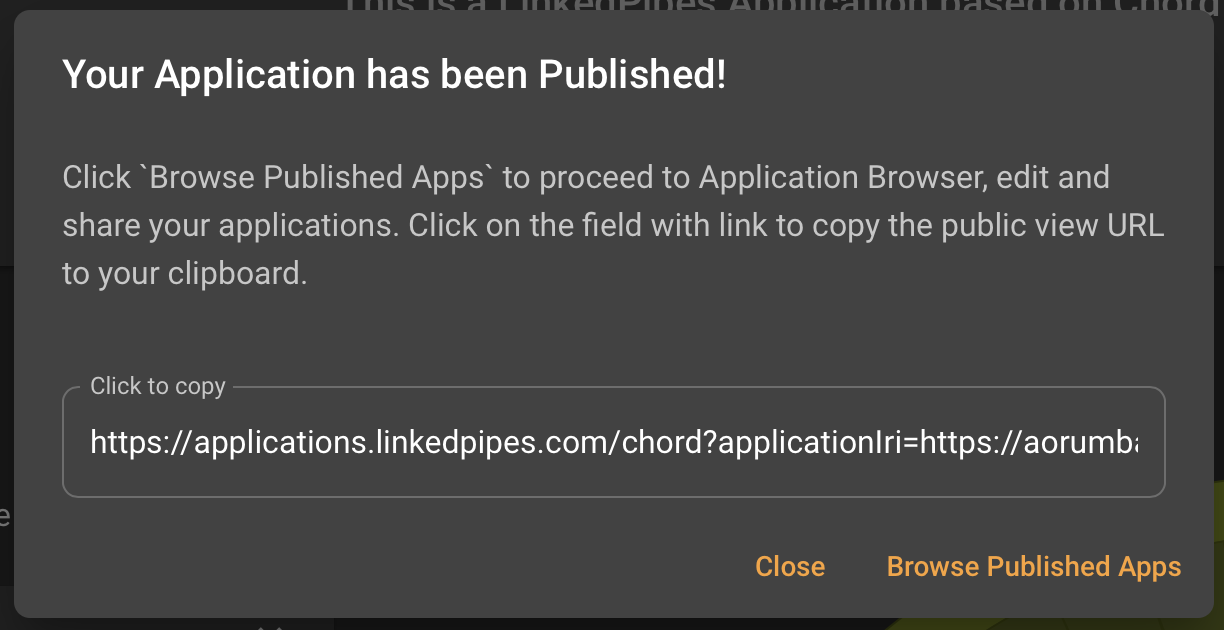
\includegraphics[width=0.8\linewidth]{lpa_published_popup.png}}
\caption{A popup presented after configuration is stored and a published url is ready to be shared.}
\label{fig:lpa_published_app_popup}
\end{figure}

This concludes the demonstration of components and functionality of both \lpa{} and \lpas{} package that implement the functional requirements on storing, publishing and creating \lpa{} configurations. 

\subsection{Configuring Application}
\label{ssssec:configuring_application_implementation}

The ability to configure the published applications had a clear and straightforward set of terms to implement. After publishing an application \lpa{} users  to \textit{rename}, \textit{delete} the configuration as well as configure and modify the filters available for the visualiser.

\subsubsection{Renaming application}

Renaming the published application is performed by executing a simple \texttt{SPARQL} query. The \textit{fetch()} method available in \textit{AuthenticationManager} abstraction from \lpas{} package is used to send the constructed request. 

\begin{listing}[H]    
\begin{minted}[breaklines,frame=single,framerule=1pt,bgcolor=LightGray]{javascript}
const sparqlQuery = `
        @prefix lpa: <https://w3id.org/def/lpapps#> .

        DELETE
        { ?configuration lpa:title ?titleValue . }
        INSERT
        { ?configuration lpa:title "${newTitle}" .}
        WHERE
        { ?configuration lpa:title ?titleValue . }
`;
\end{minted}
\caption{An example of \texttt{SPARQL} query to update the application title in configuration stored in \solid{}.} 
\label{lst:lpapp_sample_rename_app_sparql}
\end{listing}

Example on \autoref{lst:lpapp_sample_rename_app_sparql} demonstrate the \texttt{SPARQL} query used for renaming the title of \lpa{} configuration. The source code on \autoref{lst:lpapp_patch_file_with_query} demonstrate how the query is constructed and submitted to \solid{} using a class called \textit{StorageSparqlClient}.

\begin{listing}[H]    
\begin{minted}[breaklines,frame=single,framerule=1pt,bgcolor=LightGray]{javascript}
patchFileWithQuery = async (url, query) => {
  try {
    await StorageAuthenticationManager.fetch(url, {
      method: 'PATCH',
      body: query,
      headers: {
        'Content-Type': 'application/sparql-update'
      }
    });
    return true;
  } catch (error) {
    if (error instanceof Response && error.status === 404) return false;
    throw error;
  }
};
\end{minted}
\caption{The \textit{patchFileWithQuery} method in \textit{StorageSparqlClient} class is used for executing the PATCH requests to \solid{} servers.} 
\label{lst:lpapp_patch_file_with_query}
\end{listing}

\begin{figure}[h]
\centering
\fcolorbox{black}{white}{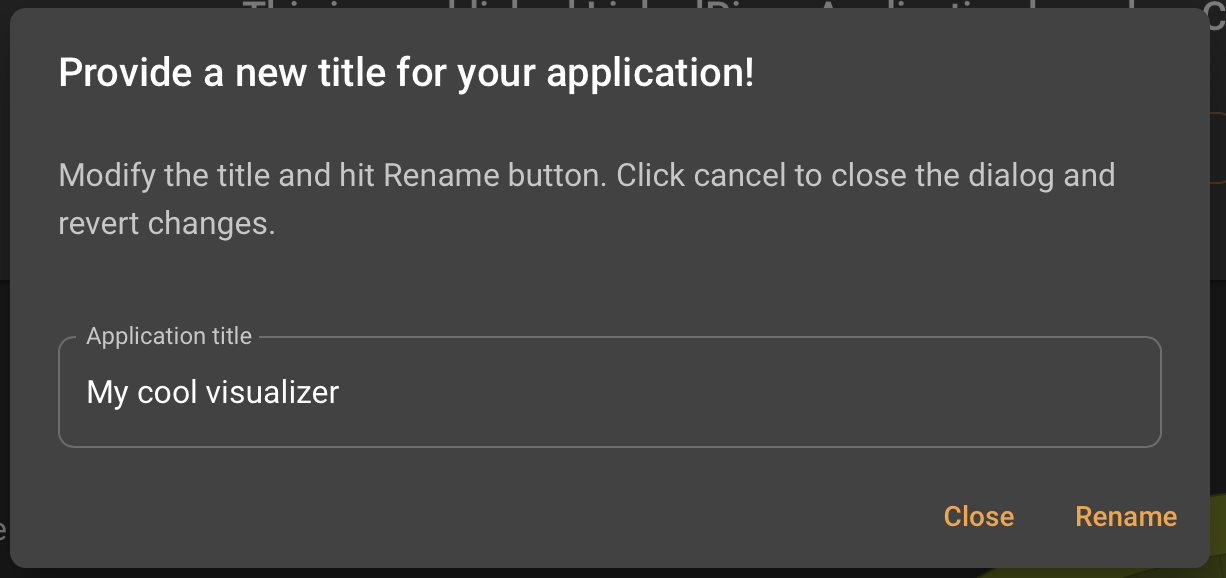
\includegraphics[width=0.8\linewidth]{lpa_rename_visualzer.png}}
\caption{A popup presented after user pressed \textit{Rename} button.}
\label{fig:lpa_rename_visualzer}
\end{figure}

On the frontend side, the rename is invoked by pressing the \textit{Rename} button from the \textit{Application Control and Setup} webpage. The user is presented with a simple popup dialog demonstrated on \autoref{fig:lpa_rename_visualzer}, where he gets an option to choose the new title of his application. This invokes the execution of the \texttt{SPARQL} query mentioned earlier.

\subsubsection{Deleting application}

Deleting an application that was previously published is a trivial task from the standpoint of \lpas{}. When user wants to delete the application he simply invokes the \textit{Delete} button either from individual application card in \textit{Storage Dashboard} webpage or inside the \textit{Application Control and Setup} webpage. Executing the deletion invokes the \textit{StorageToolbox} class that uses the \textit{deleteResource()} function from \textit{FileManager} abstraction in \lpas{} package described in \autoref{sssec:file_manager_implementation}.

\begin{figure}[hbt]
\minipage{0.3\textwidth}
  \fcolorbox{black}{white}{
\includegraphics[width=0.8\linewidth]{lpa_delete_from_configuration_page.png}}
  \caption{Option to invoke the deletion confirmation popup on \textit{Application Control and Setup} web page}
  \label{fig:lpa_delete_from_configuration_page}
\endminipage\hfill
\minipage{0.6\textwidth}
  \fcolorbox{black}{white}{
\includegraphics[width=0.8\linewidth]{lpa_delete_app_confirmation.png}}
  \caption{Popup displayed before removing published application configuration.}
  \label{fig:lpa_delete_app_confirmation}
\endminipage\hfill
\end{figure}

The popups that appear to user when he presses the \textit{Delete} button on \autoref{fig:lpa_delete_from_configuration_page} is presented on \autoref{fig:lpa_delete_app_confirmation}.

\subsubsection{Updating filters}
\label{ssssec:updating_filters_implementation}

The ability to modify the filters on a published visualizer is another important part of the \textit{Configure Application} functional requirement. The process of updating filters on published applications is invoked when a user modifies available \textit{node} or \textit{scheme} filters. For example, the UI elements on \autoref{chap:num_1} demonstrate a \textit{CHORD} visualizer containing multiple \textit{node} filters. User has an option to control \textit{state} of the filter, \textit{visibility} to the end user and \textit{interactivity} or the ability for public viewers to interact with the visualizer using the individual filters. 

\begin{figure}[h]
\centering
\fcolorbox{black}{white}{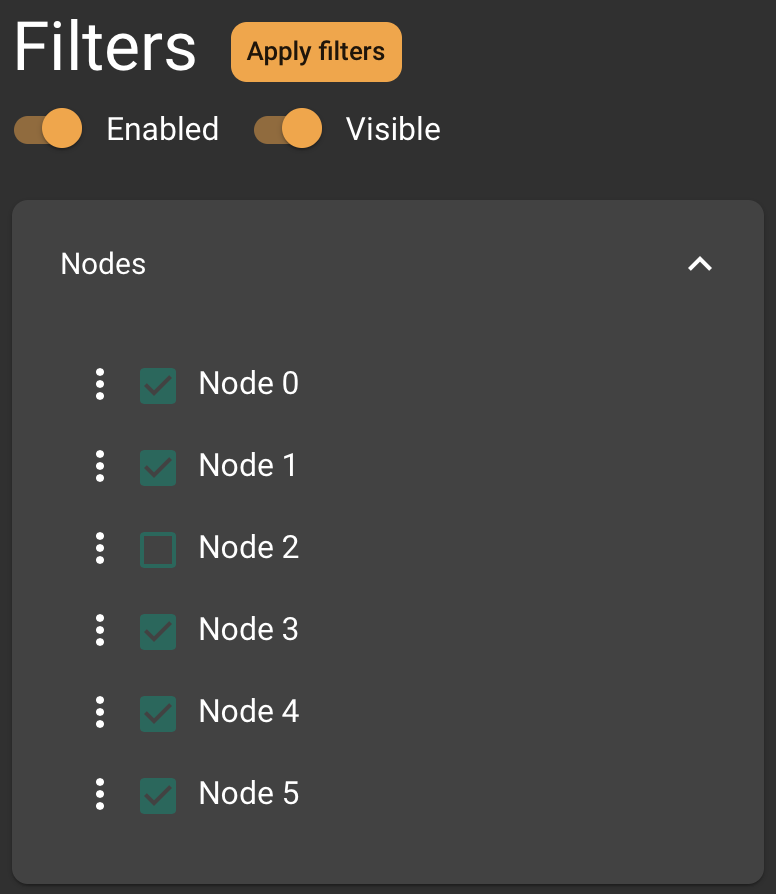
\includegraphics[width=0.5\linewidth]{lpa_filters_ui.png}}
\caption{A user interface components to interact with filters available for a visualizer.}
\label{fig:lpa_filters_interactions}
\end{figure}


The implementation of methods processing these operations are done in \textit{StorageToolbox}, \textit{StorageBackend} and \textit{StorageSparqlClient} classes, and similar to \textit{Renaming Application} procedure, the core logic simply constructs the required \texttt{SPARQL} queries and executes them using HTTP PATCH request. Example on \autoref{lst:lpapp_sample_set_filter_sparql} demonstrates the construction of \texttt{SPARQL} query that processes multiple filter selections in a single PATCH call.  

\begin{listing}[H]    
\begin{minted}[breaklines,frame=single,framerule=1pt,bgcolor=LightGray]{javascript}
let sparqlQuery = '@prefix lpa: <https://w3id.org/def/lpapps#> .';
const deleteStatements = [];
const insertStatements = [];
const whereStatements = [];

for (const node of nodes) {
  deleteStatements.push(`?selectedOption${cnt} lpa:uri "${node.uri}" .
  ?selectedOption${cnt} lpa:selected ?selected${cnt} .
  ?selectedOption${cnt} lpa:visible ?visible${cnt} .
  ?selectedOption${cnt} lpa:enabled ?enabled${cnt} .`);

  insertStatements.push(`?selectedOption${cnt} lpa:uri "${node.uri}" .
  ?selectedOption${cnt} lpa:selected "${node.selected}" .
  ?selectedOption${cnt} lpa:visible "${node.visible}" .
  ?selectedOption${cnt} lpa:enabled "${node.enabled}" .`);

  whereStatements.push(`?selectedOption${cnt} lpa:uri "${node.uri}" .
  ?selectedOption${cnt} lpa:selected ?selected${cnt} .
  ?selectedOption${cnt} lpa:visible ?visible${cnt} .
  ?selectedOption${cnt} lpa:enabled ?enabled${cnt} . `);
}

sparqlQuery += `
  DELETE { ${deleteStatements.join('\n')} }
  INSERT { ${insertStatements.join('\n')} }
  WHERE { ${whereStatements.join('\n')} }
`;
\end{minted}
\caption{An example of \texttt{SPARQL} query to update the state of multiple \textit{node} filters selected by user.} 
\label{lst:lpapp_sample_set_filter_sparql}
\end{listing}

One of the additional features implemented within the bounds of that requirement is the ability to reflect the applied changes in any field of the application configuration RDF file using socket listeners. In other words, if a user is editing filters on his visualizer and some other user is looking at his visualizer on some webpage where it is published, he will see the changes being applied in real-time. This is implemented using the \texttt{rdflib.js} library that is accessed via \lpas{} package. The \autoref{lst:lpap_add_listeners_function} demonstrates a simple utility function available at \textit{StorageBackend} and it is invoked when application configuration is being fetched for the first time. 


\begin{listing}[H]    
\begin{minted}[breaklines,frame=single,framerule=1pt,bgcolor=LightGray]{javascript}
registerChanges(url: string, callbackOnRefresh: Function = undefined) {
  if (this.alreadyAddedDownstreamListeners.indexOf(url) === -1) {
    const doc = $rdf.sym(url).doc();
    this.updater.addDownstreamChangeListener(doc, callbackOnRefresh);
    this.alreadyAddedDownstreamListeners.push(url);
  }
}
\end{minted}
\caption{Implementation of helper utility that uses feature of \texttt{rdflib} to invoke any callback when a change in a specified RDF resource is detected.} 
\label{lst:lpap_add_listeners_function}
\end{listing}

\subsection{Storage Management}

The Storage Management functional requirement defines an implementation request to have an ability to \textit{move}, \textit{rename} or \textit{copy} the root folder with all configurations inside the storage. From the perspective of \lpas{} it implies controlling the root LDP Basic Container that stores all configurations.

\begin{figure}[h]
\centering
\fcolorbox{black}{white}{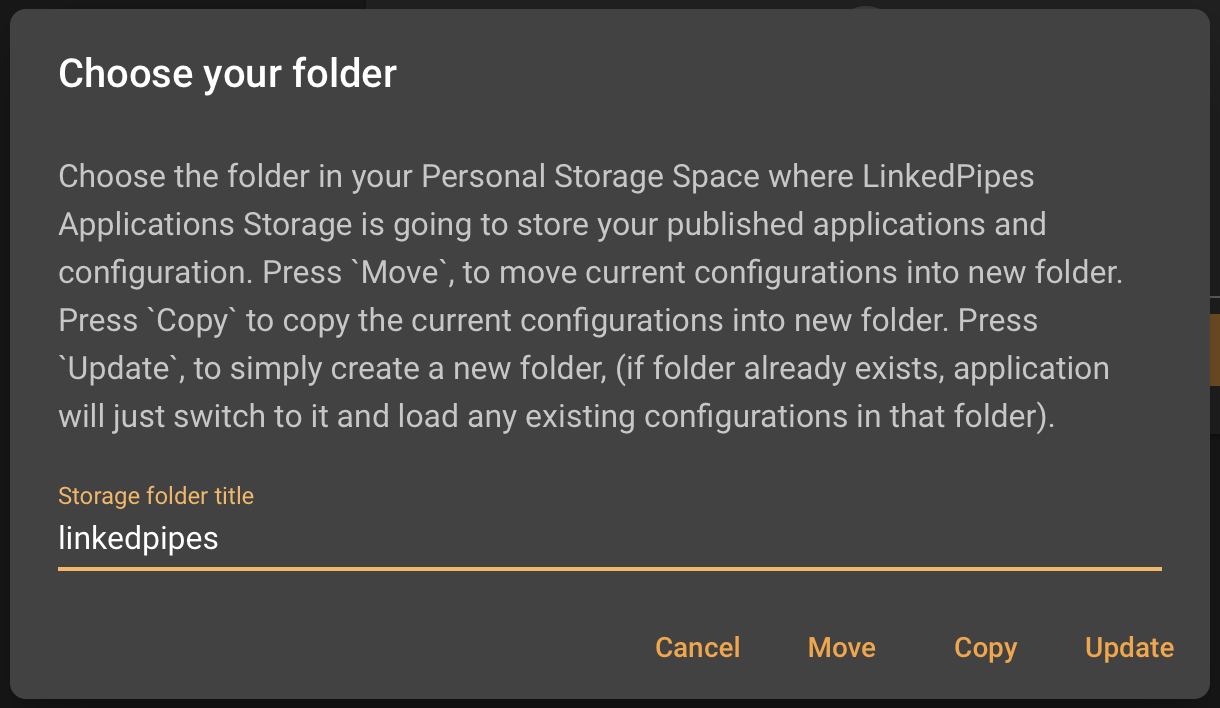
\includegraphics[width=0.7\linewidth]{lpa_updating_root_folder.png}}
\caption{A final render of Storage Control Panel component.}
\label{fig:lpa_updating_root_folder}
\end{figure}

Since the description in \autoref{sssec:storage_control_panel_implementation} already provided all details on implementing this requirement, this section will demonstrate the final renders of implemented components to perform the operations stated in the requirement. The user interface demonstrated on \autoref{fig:lpa_updating_root_folder}, performs the functionality as requested in the definition of the requirement. It is invoked via \textit{Settings} webpage under \textit{Application Storage} tab when user clicks on \textit{Change folder} tab. 

\subsection{Visualizer Access Control}

The Visualizer, Access Control requirement, defines how the creator of an application can control public access to visualizer or share it with only a specified set of contacts. From the \lpas{} standpoint, this implies controlling the ACL files of individual \lpa{} configurations expressed in RDF.

\begin{figure}[h]
\centering
\fcolorbox{black}{white}{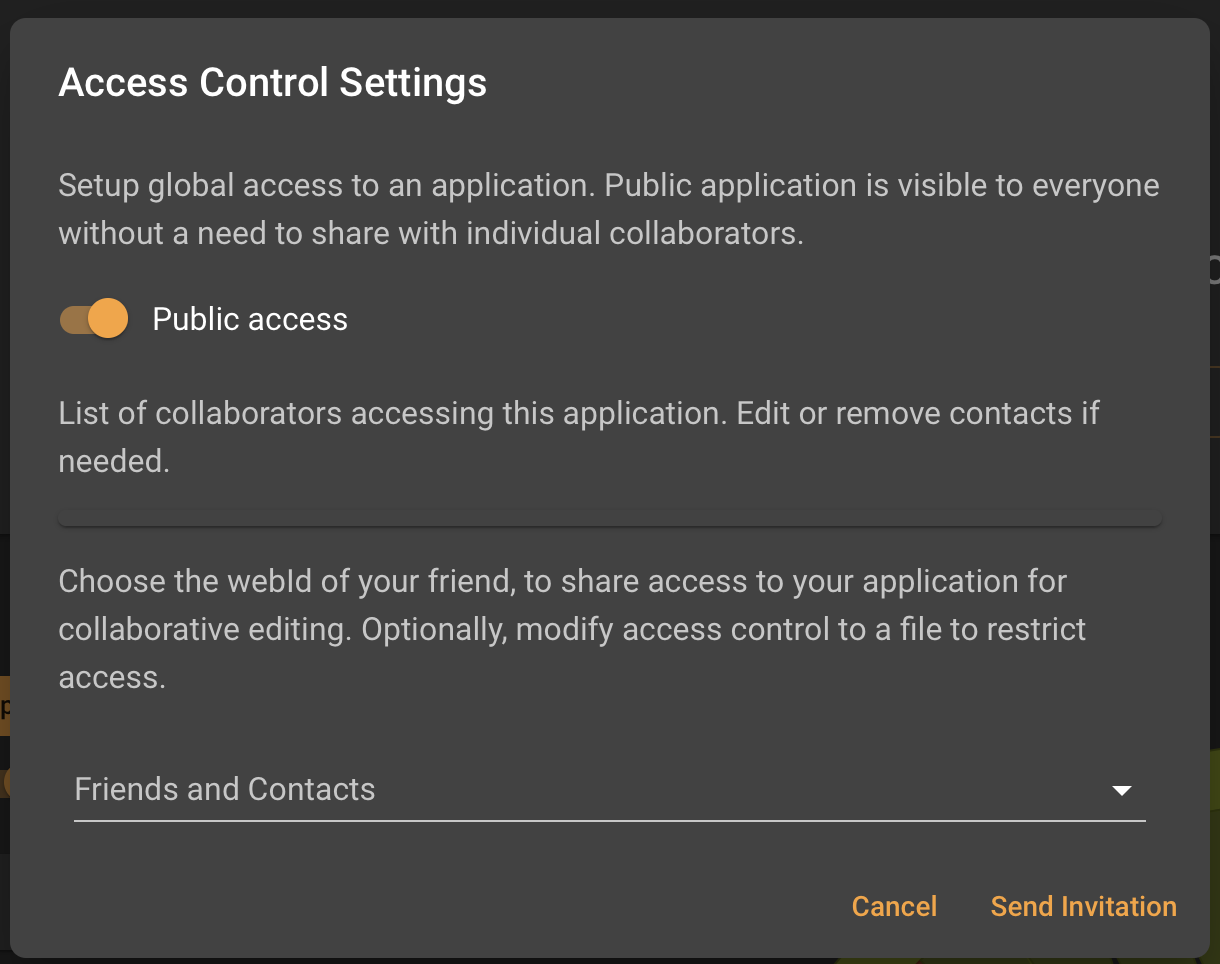
\includegraphics[width=0.7\linewidth]{lpa_access_control_setup.png}}
\caption{Access control configuration popup for published application.}
\label{fig:lpa_access_control_setup}
\end{figure}

The implementation of \textit{AccessControlManager} abstraction in \autoref{sssec:access_control_manager_implementation} is the essential building block that was used to implement a set of React Components to allow modifying access control privileges of published visualizers. The \autoref{fig:lpa_access_control_setup} demonstrate an final render of a React Component that is presented to user when he clicks on \texttt{Access Control} drop down item on \textit{Application Control and Setup} webpage. The component is implemented in \textit{StorageAccessControlDialog} file which is a simple stateful React Component. The main elements of that popup can be described as follows:
\begin{itemize}
    \item \textit{Public access} switch, this element controls the default public access to a published application. By default, \lpa{} sets the \textit{READ} public access so that anyone can access the published application by default. However, the user has an option to toggle the control element and disable default public visibility. 
    \item \textit{List of collaborators}, this element lists the contacts knows to user's \textit{WebID}. The querying of knows contacts is performed using \texttt{rdflib} library accessed via \lpas{} package. 
    \item \textit{Friends and Contacts} dropdown, this element is a selector for sending invitations to share the published visualizer with other users of the platform. The next subsection will provide more details on the collaborative sharing feature implemented as an additional functionality on top of the initial functional requirement. Collaborative sharing features implementation is inspired by \textit{\gls{LDN}} \cite{ldn} and uses the \textit{ActivityStreams} vocabulary \cite{activitystreams}. However, due to the specificity of \lpa{}, it does not strictly follow all requirements of that specification. 
\end{itemize}

\subsubsection{Collaborative sharing}
\label{ssssec:collaborative_sharing}

Collaborative sharing allows users of \lpa{} platform to share their visualizers with other users of the platform. The sharing process implementation is inspired by Linked Data Notifications specification \TODO{cite here} and involves the generation of an invitation file that send to the recipients inbox. The \autoref{fig:lpas_sharing_application} demonstrates the process of submitting an invitation in detail.

\begin{figure}[h]
\centering
\fcolorbox{black}{white}{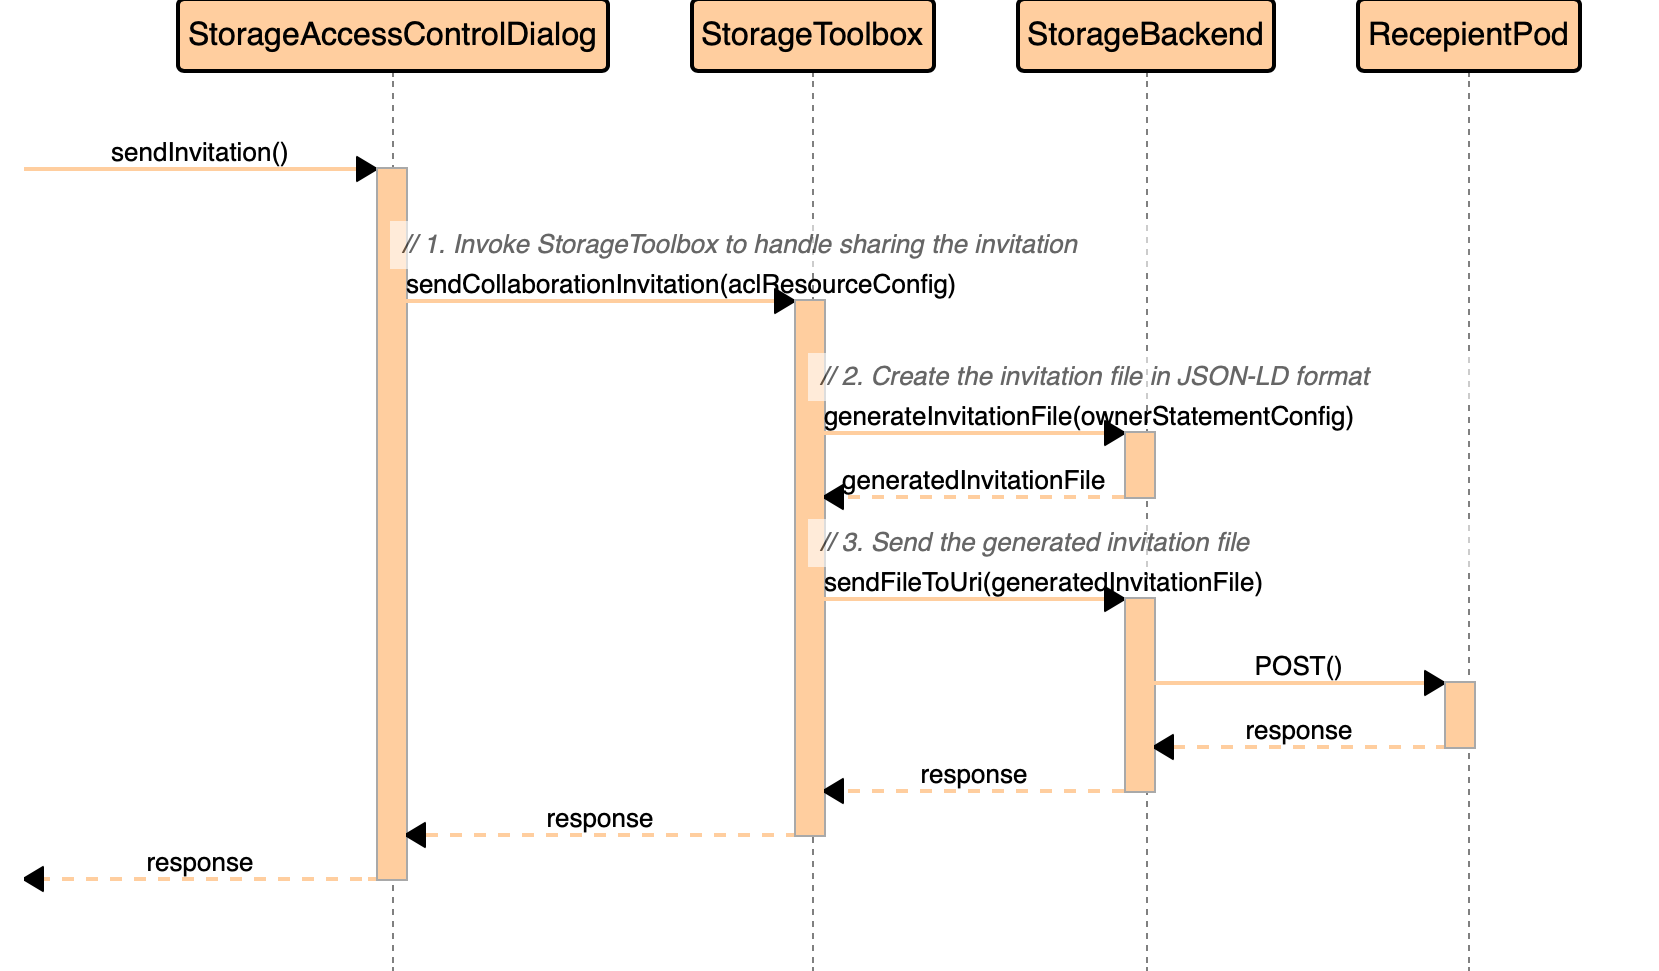
\includegraphics[width=0.8\linewidth]{lpas_sharing_application.png}}
\caption{A sequence diagram of implemented sharing functionality for collaborative editing.}
\label{fig:lpas_sharing_application}
\end{figure}
  
The steps can be described as follows:
\begin{enumerate}
    \item Firstly, the \textit{sendInvitation()} function is invoked from \textit{StorageAccessControlDialog} React Component, specifically when users chooses his available list of contacts and presses submit invitation button.
    \item As a next step, \textit{StorageToolbox} redirects the request to lower-level \textit{StorageBackend} class.
    \item The \textit{StorageBackend} class generates the invitation RDF in JSON-LD format using \texttt{rdflib} library from \lpas{} package.
    \item The \textit{StorageBackend} class sends the invitation file to recepients inbox folder using \textit{FileManager} abstraction from \lpas{} package. The exact inbox path is known by parsing the recipient's profile card associated with his WebID.
    \item Asyncronous response is returned of the operations is propagated back to \textit{StorageAccessControlDialog} for further processing. 
\end{enumerate}
 
\begin{figure}[h]
\centering
\fcolorbox{black}{white}{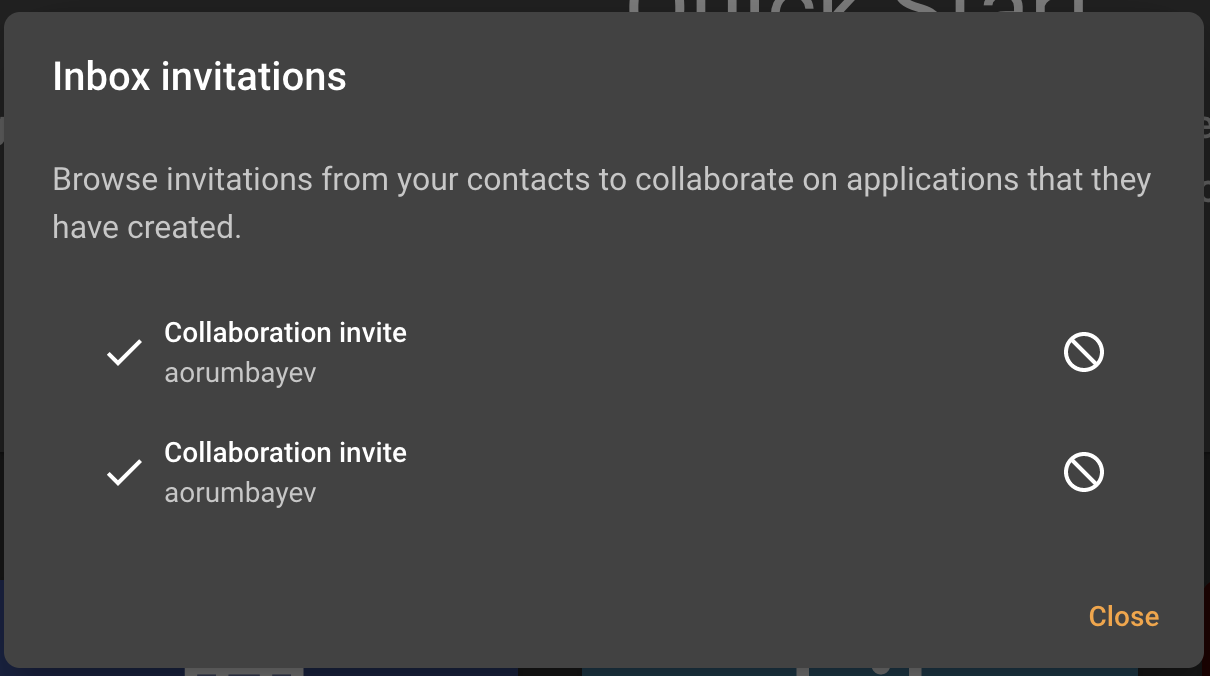
\includegraphics[width=0.7\linewidth]{lpa_inbox_with_invitations.png}}
\caption{An inbox dialog popup with two new invitations to collaborate on application.}
\label{fig:lpa_inbox_with_invitations}
\end{figure}
  
 
It is important to note that the recipient is assumed to be a user of \lpa{} platform. Once invitation is send, whenever recipient opens the platform, the listener inside \textit{AppRouter} class will check the inbox for new invitations and display new invitations in inbox popup demonstrated on \autoref{fig:lpa_inbox_with_invitations}. If user \textit{Accepts} the invitation, the invitation JSON-LD file is transformed into a shared configuration file by extracting URI to an application and placing it under a folder named \textit{sharedApplications} in the root storage folder and a response notification is sent back to the sender. Once sender receives the \textit{Accept} notification, it sets the \textit{READ} and \textit{WRITE} access to the application configuration for the recipient. If user \textit{Declines} the invitation, the invitation is deleted from the inbox without any further processing.

\begin{figure}[h]
\centering
\fcolorbox{black}{white}{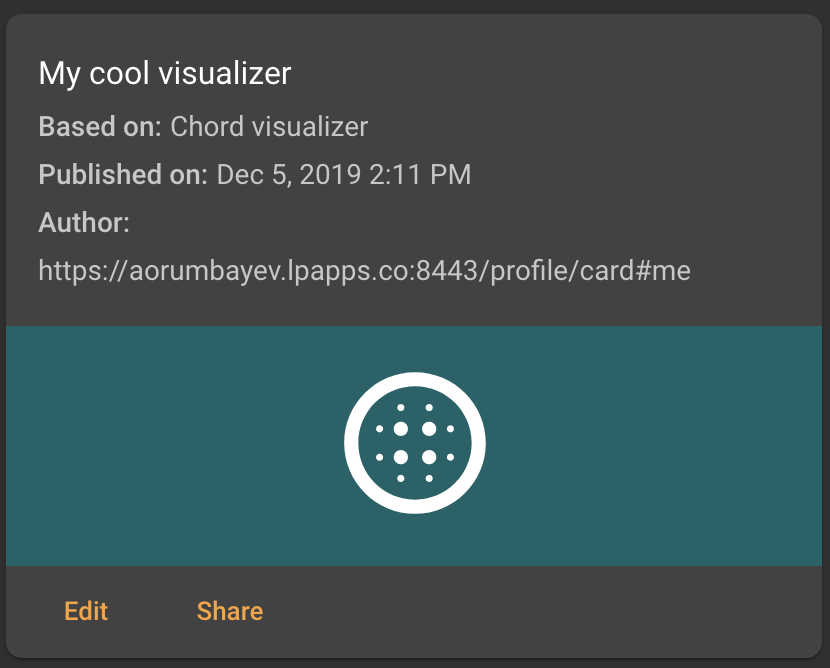
\includegraphics[width=0.7\linewidth]{lpa_shared_visualizer_card.png}}
\caption{A shared visualizer card displayed to recipient in his Storage Dashboard after he accepts the invitation.}
\label{fig:lpa_shared_visualizer_card}
\end{figure}

The \autoref{chap:num_1} demonstrates the shared application appearing in the shared applications storage dashboard of the recipient. In addition to that, the code on \autoref{lst:lpa_example_invitation_json_ld} demonstrates the example of the generated invitation being send to recipient in JSON-LD format using \textit{ActivityStreams} vocabulary. 

\begin{listing}[H]    
\begin{minted}[breaklines,frame=single,framerule=1pt,bgcolor=LightGray]{json}
{
  "@context": "https://www.w3.org/ns/activitystreams",
  "type": "Invite",
  "actor": "https://sender.lpapps.co:8443/profile/card#me",
  "name": "lpapps_invite",
  "object": {
    "type": "Link",
    "href": "https://sender.lpapps.co:8443/
    linkedpipes/configurations/1575551497789.473.ttl"
  },
  "published": "2019-12-06T20:04:02Z",
  "target": "https://recipient.lpapps.co:8443/profile/card#me"
}
\end{minted}
\caption{An example invitation to collaborate on a published application.} 
\label{lst:lpa_example_invitation_json_ld}
\end{listing}

The collaborative aspect is basic and only allows the recipient to rename the title of the application and modify and persist the selection of available filters. The changes are reflected in real-time using socket connection to \solid{} server as initially described in \autoref{ssssec:updating_filters_implementation}.

To sum up, the following section iterated over each functional requirement stated by \lpa{} and demonstrated the detailed description of implementation to comply with those requirements. The section also continued the storage-related React Components implementation details provided in \autoref{sssec:lpas_storage_frontend_implementation} and demonstrated finalized renders of those components that closely follow the initial mocks designed in \autoref{chap:num_4}. 

\section{Implemented non-functional requirements}
\label{ssec:non_functional_requirements_implementation}

The section provides a general overview of implementation of non-functional requirements stated in \autoref{ssec:non_functional_requirements}. Due to the majority of requirements being covered simply by the core functionality of the \solid{} project itself the implementation details of individual requirements are less descriptive than descriptions in \autoref{ssec:overview_of_implemented_requirements}. It is also important to note that this section provides the implementation overview of all stated functional requirements defined in \autoref{ssec:non_functional_requirements}.

\subsection{Compatibility with latest tools}

The implemented solution consists from three parts:
\begin{itemize}
    \item The \lpas{} package, an npm package containing the generic abstractions performing low-level interactions with instances of \solid{} servers. Relies on \texttt{rdflib}, \texttt{solid-auth-client} and \texttt{solid-auth-cli} libraries. All third party packages are pinned, stable and indirectly unit tested, more details on testing is provided in \autoref{chap:num_7}. 
    \item The Storage React components, a set of frontend components written in ES6 inside the \lpa{} package. No additional third party packages are introduces to \lpa{} with these components, except for \lpas{} package. 
    \item The \lpas{} ontology, a vocabulary designed with \texttt{Protégé} and published with \texttt{Ontoology}. Used in \lpa{} by accessing its public hosted instance, therefore no additional third party packages are introduced.
\end{itemize}

\subsection{Clean APIs and libraries}

The whole intent of creating the \lpas{} package was to refactor and redesign the abstractions interacting with solid inside \lpa{} frontend codebase. Therefore, the final refactored implementation is easier to maintain and use by LPA developers due to usage of TypeScript, extensive automated testing coverage covered in \autoref{chap:num_7}, and documentation included in \autoref{chap:num_8}.

\subsection{Continuous Integration and Delivery}

The \lpas{} package is located in a separate GitHub repository, has an automated continuous delivery pipeline invoking unit test, code formatting, and linting. The continuous delivery aspect publishes new npm versions in is semi-automated manner. The frontend storage components in \lpa{} are incorporated into frontend codebase. Hence they are validated using the \lpa{} CI and CD pipelines. Some improvements into \lpa{} testing pipelines were introduced, and they are described in detail in \autoref{chap:num_7}.

\subsection{Easy integration with \lpa{}}

The \lpas{} package is distributed via npm, and seamlessly integrated into \lpa{} using the package management software. The frontend storage components are implemented inside the frontend codebase. However, they also maintain a consisted structure that improves code readability and defines the logical separation between functionalities of \lpa{} and \lpas{}.

\subsection{Decentralized storage}

The solution for this non-functional requirement is covered by \solid{} specification. Since \solid{} servers are decentralized by design, it means that the \textit{AuthenticationManager} from \lpas{} package allows the users of \lpa{} to authenticate with any arbitrary instance of their private \solid{} server instances or instances from third-party \solid{} providers. The \textit{FileManager} abstraction also allows users to move the created \lpa{} configurations between \solid{} PODs within a \solid{} server instance or between different instances of compatible \solid{} servers.